
\documentclass[doctor,english,listoffigures,listoftables]{thesis-uestc}
\usepackage{algorithm} 
\usepackage{algpseudocode} 
%%\usepackage{multirow,hhline,pstricks,color,wasysym,marvosym,mathptmx,longtable,subcaption,graphicx,float}
%%\usepackage[T1]{fontenc}

%%\usepackage{textcomp,booktabs}
%\usepackage{adjustbox}
%\usepackage[usenames,dvipsnames]{color}

\title{The Study of The Key Techniques on Single Image Dehazing.}

\author{************}{Jehoiada ************}
\advisor{Professor ******}{Professor ******}
\school{信息与软件工程学院}{School of Information and Software Engineering}
\major{软件工程术}{Software Engineering}
\studentnumber{201******}

\begin{document}

\makecover

\begin{chineseabstract}
大气颗粒的自然和不自然散射会极大地影响在露天环境中******。

\begin{enumerate}
	\item ******。 
	
	\item ******
	
	\item ******果。
	
	

	
\end{enumerate}
通过对模糊图像进行的大量定性和计算实验表明,所提出的方法在实现更快的处理时间的同时,可以产生了出色的结果。

\chinesekeyword{图像去雾,瑞利散射,透射图, 残差网络,暗通道}
\end{chineseabstract}

\begin{englishabstract}
The****** 
\begin{enumerate}
	\item   ******************************
	\item  ************************ 
\end{enumerate}
Overall, an extensive qualitative and computational experiments on hazy images demonstrate that the proposed method produces excellent results whiles achieving a faster processing time.

\englishkeyword{Image dehazing, Rayleigh scattering, Residual network, CNN, Dark Channel.}
\end{englishabstract}

\thesistableofcontents
\thesisfigurelist
\thesistablelist
\thesischapterexordium

This chapter introduces the framework of the image dehazing problem, including the physical degradation model widely adopted. 

\section{Research Background}
An image comprises a matrix with square pixels aggregated of rows and columns. Images are classified as grey scale or color. That is, they do not represent any color, only the level of brilliance for one color. An image consists of only 8 bytes 256(0-255) levels of illumination, 0 is for dark, and 255 is white. In the middle are numerous levels of brightness. The colored image contains red, green, and blue (RGB) groups, each having 8 bytes of intensity. The changing intensity levels in each band can pass on the whole colored image making 24bit. Digital image processing is a universal topic and involves procedures that can be scientifically changeable, but digital image processing focal idea is straightforward. The whole goal of digital image processing is to appropriate the image’s information to enable the system to understand, recognize and translate the processed data obtainable from the image pattern. Digital imaging has mutated into a vital element of our everyday lives; images with excellent contrast and brightness are essential in our daily lives. Images are needed in broad research fields: medical imaging, criminological analysis, monitoring, universal identity affirmation. Image enhancement is a strong motivation in computer vision and has received enormous concentration. The ultimate objective of Image enhancement is to restore images to produce a more helpful contribution for other automated image processing steps, such as research, detection, segmentation, and recognition. In recent years computerized cameras are unquestionably the most utilized devices to obtain images. However, the properties of images captured sometimes are distorted and have low contrast. 
\section{Problem Statement}
Images captured in an open-air environment usually are influenced by natural and unnatural adverse weather conditions such as smoke, haze, and smog due to visibility-reducing aerosols, which considerably generates the color change and reduces the contrast of the image. These Aerosols occur when there is a complex chemical reaction between the atmosphere and the chemical compound, sulfur dioxide gas $(SO_2)$ to produce tiny sulfuric acid molecules ($H_2SO_4$)\citing{a1,a2}. Haze is a joint event on land and the ocean. In a hazy climate, there are many atmospheric particles of vital size. The presence of sunshine, high liquidity, and stagnant airflow may strengthen the formation of aerosols. This phenomenon is a significant problem in computer vision and consumer photography, as shown in Figure~\ref{fig1}. Haze removal algorithms have achieved significant attention in the computer technology area. They have broadly been applied in public and military domains, such as remote sensing, object detection, traffic monitoring, and image quality evaluation. For outdoor images, Narasimhan et al.\citing{a26} examined the visible displays of varying weather conditions, such as haze, fog, cloud, and rain, and then discovered an imaging degradation model on the climatic scattering appearance for image dehazing. Numerous enhanced haze removal algorithms based on the physical model were proposed based on outdoor images. However, there are fewer studies on images obtained from the sea and air. The above applications all explain that the Image dehazing algorithms are essential and completely meriting studying.

\begin{figure}[H]
	\centering
	\includegraphics[width=5.5in]{1.png}
	\caption{ Atmospheric Scattering model.}
	\label{fig1}
\end{figure}
Image dehazing has two purposes: (1) advancing the visibility scene and obtaining the loss of light intensity created by visible aerosols.(2) improving consumer photography and computer vision application\citing{a3,a4}. However, dehazing is an ill posed problem in computer vision and image processing due to its dependency on unknown scene depth. 
\begin{figure}[H]
	\centering
	\includegraphics[width=5.7in]{2.png}
	\caption{ Variables in the haze degradation model. The transmission map t is shown as white when t=1 and black when t=0.}
	\label{fig2}
\end{figure}
In the computer vision domain, the model universally accepted in the creation of haze is the atmospheric scattering model, and it has two principal components\citing{c11,c12}: (I) linear attenuation of light reflected from the scene to the camera. (II) the volume of scattered light that enters the camera. The model illustrates that haze formation is a convex fusion of air light and the direct attenuation, as shown in Figure~\ref{fig2}. The model can be formulated as\citing{a5}:
\begin{equation}\label{scattering}
	I{(x)}=J{(x)} t{(x)} + A(1-t{(x)}),
\end{equation}

where $J$ depicts the scene radiance of the image, $J{(x)}$ is a 3D vector coordinates of the RGB color channel reflected by the scene point at $x$. The scene radiance is the amount of light the observe should see in the absence of haze, as shown in Figure~\ref{fig3}. The 2D vector coordinates of a pixel's location in the image is represented by $x$. $I$ is the observed intensity in each RGB color channel. $t$ is the transmission map or transparency of the haze. $t{(x)}$ is a scalar in [0, 1]. Intuitively, if $t = 1 $ the light is unscattered and completely clear but when $t = 0 $ incoming light disperses which indicates there is haze. In semi transparent transmission map $t$ is represented as $0 < t{(x)} < 1$ as shown in Figure~\ref{fig2}. The atmospheric light, which is the color of the sky areas, is represented by $A$. The first term of the equation $J{(x)} t{(x)}$ is called direct attenuation, which describes partially absorbed light by atmospheric particles reflected from the object scene\citing{c13,c14,AN1,AN2}. The last term $A(1-t{(x)})$ is called airlight. The airlight is the unlimited amount of light origin resulting from the scattering of light by atmospheric particles. The sky is not a concrete object; therefore, recreating the atmospheric effect is challenging\citing{a6,a7,a8}. An object scene under atmospheric scattering is affected by the amount of airlight it travels on; for instance, A mountain seen from a range seems to blend with the sky due to a comparatively low air density on earth. 

\begin{figure}[H]
	\centering
	\includegraphics[width=5.5in]{3.png}
	\caption{ In-scattering ray of light deflected towards the camera.}
	\label{fig3}
\end{figure}

When light diverges by aerial particles, it is redirected towards the camera, forming halos around the light's origin. The haze formation model possesses several unknown parameters which equate to the number of pixels in an image. Considering that the transmission map $t$ is the equivalent for each RGB color channel, the total number of unknowns is 4N + 3, much greater than the number 3N of equations\citing{a9,a10}. In computer vision, we refer to this difficulty as under constrained. In this way, the direct estimation of the transmission map $t{(x)}$ from the observed intensity $I{(x)}$ is restrictive with no earlier postulates. The recovery of the scene radiance $J$ becomes apparent once the transmission map $t{(x)}$ and atmospheric light $A$ are calculated\citing{a11}:
\begin{equation}\label{scene}
	J(x)=\frac{I(x)-A(x)(1-t(x))}{t(x)}
\end{equation}
In a uniform atmosphere, the transmission map $t$ is formulated as:
\begin{equation}\label{scattering}
	t(x)=e^{-\beta d(x)},
\end{equation}
where $\beta$ denotes the attenuation coefficient based on the wavelength, and the scene depth is represented by $d$.
To address the constraint problems the haze degradation model presents, we categorize the solution into three strategies: (I) Multiple know variables strategies, (II) Prior based strategies, and (III) CNN-based strategies. In the first strategy, multiple images captured under the same scene at different climate conditions are utilized to obtain a haze free image. The second strategy utilizes heuristic assumptions in achieving a haze free image. The final approach, which is the most current algorithm, attains a haze free image by using a deep convolutional neural network (CNN).

\section{Contribution and Significance. }
In summary, this dissertation presents the design and implementation of (I) A robust Prior algorithm, (II) a deep convolutional neural network, and (III) real time contrast enhancement models for achieving haze free images. This work primarily has three significant contributions:

\begin{itemize}
	\item A compelling Single image dehazing algorithm based on dark channel prior and Rayleigh scattering. This algorithm estimates the atmospheric light through the computation of average, minimum, and maximum pixels in each of the three color channels. Using the theory of Rayleigh scattering, we model a scattering coefficient to estimate the initial transmission map. A fast guided filter is also adopted to refine the initial transmission map due to inaccurate halo edges. Finally, we restore the haze free image through the atmospheric scattering model.  
	
	\item A robust CNN based dehazing algorithm. The proposed algorithm is non-subject to the climatic dispersing model, yet it learns the mapping relationship within the hazy input image and their corresponding transmission map. The network architecture constitutes a convolution kernel and multi-scale fusion layers in extracting relevant features in predicting a holistic propagation map. Ultimately, we obtain the residual image and circumvent the loss of information using a residual network. We synthesize a dataset comprising of hazy pictures and their identical transmission map from the NYU Depth dataset to train the network.
	
	\item An efficient real-time single image dehazing algorithm. The algorithm's basis is on Histogram and a filtering manipulation on the lab color channel. In the proposed algorithm, the input RGB image is transformed into Lab color channel then, contrast limited adaptive histogram equalization(CLAHE), and a smoothing operation is applied respectively and simultaneously on the luminosity layer and the other two-color channels of the Lab color space. We merge the channels to obtain a new enhanced image. 
	
\end{itemize}

\section{Outline of the Thesis}
Following the introduction, the remainder of the dissertation is summarized as follows: 

\begin{enumerate}
	\item \textbf{Chapter 2}: This chapter provides the relevant background survey of existing literature in dehazing algorithms. The existing techniques are discussed adjacent to their advantages and drawbacks.
	\item  \textbf{Chapter 3}: This chapter presents our proposed single image dehazing algorithm using DCP and Rayleigh scattering. The algorithm estimates the atmospheric light through the computation of average, minimum, and maximum pixels in each of three color channels. Using the theory of Rayleigh scattering, we model a scattering coefficient to estimate the initial transmission map. The algorithm's implementation is described, along with adequate extensive experimental analysis.
	
	\item  \textbf{Chapter 4}: This chapter presents our CNN based algorithm for image dehazing. This end-to-end network estimates the transmission map and the atmospheric light without dependence on the atmospheric scattering model. The method outputs a propagation map medium used to recover the haze free image using a residual-based network. Extensive experimental results illustrate that the proposed technique produces a more enhanced edge-preserving image.
	
	\item  \textbf{Chapter 5}: This chapter presents our final algorithm for single image dehazing. This algorithm's basis is Histogram equalization and a filtering manipulation on lab color channel. In the proposed algorithm, we transform the input RGB night image into lab color channel then, contrast limited adaptive histogram equalization(CLAHE), and a smoothing operation is applied respectively and simultaneously on the luminosity layer " L" and the two-color channels (a and b) of the lab color space. Adequate extensive experimental analysis shows the effectiveness of our method.
	\item  \textbf{Chapter 6}: This chapter summarizes and concludes the presented methodologies and principal approaches to the dissertation. We further define potential research locus for future work within the Image dehazing domain. 
\end{enumerate}



\chapter{Theoretical Framework and Literature Review}
Chapter One presented our dissertation's problem statement using the haze effect's physical model provided by a concise haze imaging equation. This equation is the center of the entire thesis. We also express the haze removal difficulty and point out the problems.\par
Image enhancement processes consist of various procedures that endeavor to enhance an image's visible features or transform the image into a form highly satisfactory to computer vision applications. There is no universal approach to image enhancement. When an image is processed for visual analysis, the observer is the final judge of how well a particular method works. In an image enhancement system, there is no deliberate effort to improve the fidelity of a reproduced image with concern to some ideal form of the image, as is done in image restoration. Image enhancement is required in various fields of research:
\begin{enumerate}
\item In climatic sciences, image enhancement, is employed to decrease the consequences of fog, haze, fog and turbulent climate for meteorological observations. 
\item Medical imaging utilizes image enhancement procedures for reducing noise and sharpening details to enhance an image's visual representation. 
\item Image enhancement is employed by the virtual reconstruction of historical paintings and artefacts to decrease blemishes and crevices. Colour contrast enhancement, sharpening, and brightening are just some of the techniques used to brighten the images. 
\end{enumerate}

This thesis categorizes existing image enhancement techniques into two broad categories: self-enhancement and frame based fusion enhancement, according to if enhanced image embeds high quality background information. Traditional enhancement methods such as contrast enhancement method, compressed based image enhancement, and wavelet based transform image enhancement enhance low-quality images by itself\citing{a5,a7,AN3,AN4}. These approaches are uniformly called self enhancement of low quality images. In the dark image, some areas are so dark that all the information is already lost in those regions. Lost information cannot be retrieved no matter the amount of illumination enhancement you apply. Frame-based fusion enhancement refers to the fusion of extracting high quality background information to embed a low quality image. This enhancement technique borders on low quality images, which fuses illumination information in different time images. The main problem with this approach is how one would keep low-quality information while picking a high quality background. The center of this thesis would be surveyed on algorithms used in image dehazing.
In this chapter, we review earlier works on haze removal. Existing image dehazing algorithms are always instantly utilized in removing haze regardless of the appearance or absence of haze. However, it is imperative to determine if the image obtained under the current climate needs to be processed by a dehazing algorithm in real-world applications\citing{k7,k8,AN5,AN6}. This process's principal purpose is to determine if the dehazed image's clarity using dehazing algorithms may worsen than the original input hazy image\citing{a11,1,2,3}. Secondly, the process is time-consuming, which is not beneficial to realize real-time target detection, tracking, and recognition\citing{a12,AN7,AN8}. The two main methods used in assessing whether the image scene has haze in haze removal are the fog detection method, which is based on a semi-inverse image and the hazy image classification method based on the meteorological visibility reach. In haze removal literature, algorithms are classified into two sections regarding whether a physical degradation model is adopted or not \citing{a13,a14,a15,a16}. The first approach is the image restoration method based on a physical imaging model. The physical degradation model contains several parameters that must be estimated to achieve a haze free image. Image restoration algorithms aim to achieve a clear image with excellent visibility while maintaining the image's contrast. The secondary class of dehazing algorithms is based on image enhancement and does not consider the physical imaging model. This method adopts different image enhancement techniques to enhance the contrast and clarity of hazy images. The last approach is the fusion-based method, which assumes the fusion of various input images\citing{a17,a18,a19}. Figure~\ref{fig4} and Table~\ref{Tab1} shows the classification, merits, and demerits of some typical image dehazing algorithms. 
\section{Multi Image Method}
McCartney original introduced the hazy image scattering model based on the Mie scattering theory\citing{a20}. The scattering model comprises of the airlight model and direct transmission map. For a haze free image, the transmission map presents a high dimension in the physical model. The increase in the density of haze reduces the transmission map's proportion while airlight increases, reducing the image's visibility. We group the image restoration method's review into multi-image, single image, and CNN-based image algorithms on their merits and shortcomings. 

\begin{figure}[H]
	\centering
	\includegraphics[width=5.0in]{9.png}
	\caption{The categories of image dehazing algorithms}
	\label{fig4}
\end{figure}

Earlier algorithms essentially focused on using atmospheric optical features such as polarization and additional information to achieve a haze free image. This approach raises the number of identified variables, increasing the number of unknowns at an equal time. To element large unknowns, these approaches must operate under some constraints. We classify multi image dehazing algorithms into (I) Polarization based Methods, (II) Given Depth and (III) Varying Atmospheric Conditions. 
\subsection{Polarization-based Method}
This approach employs light's polarization properties to effectively remove scattered light using a polarizer (a glass filter) appended to the camera lens. In polarization-based methods, the airlight is hugely polarized, but the linear attenuation is significantly lighter. This method takes two images of the equivalent scene under two polarization events. The haze degradation equations of the two images with the assumption that the linear attenuation is unpolarized are: 
\begin{equation} \label{eq1}
	\begin{split}
		I_c^\parallel  (x) & = \frac{1}{2} J_c(x)t(x)+A_c^\parallel (1-t(x))\\
		& 	I_c^\bot (x) = \frac{1}{2} J_c(x)t(x)+A_c^\bot (1-t(x))
	\end{split}
\end{equation}
Here $\parallel $ and $\bot$ indicates two phases, and $\frac{1}{2}$ represents the factor controller of a polarizer to unpolarized light. This equation presents a total of 6N constraints, collectively with 3N unknown $J_c$, N unknown transmission map $t$, 3 unknown atmospheric light $A_c^\parallel$ and 3 unknown $A_c^\bot$ : in total 4N +6 unknown variables. Schechner\citing{a21} and Shwartz\citing{a22}, adopts the polarization method for haze elimination utilizing two or more images captured with distinct degrees of polarization displayed in Figure~\ref{fig4}. These algorithms are unwanted due to the challenge of collecting two strictly balanced polarized images. Secondly, the estimated transmission map is not frequently entirely unpolarized. Furthermore, polarization-based techniques amplify the noise of an image and are not favourable to clarity\citing{a23,a24}. 



\begin{figure}[H]
	\centering
	\includegraphics[width=5.2in]{4.png}
	\caption{ Polarization-based methods.(a1)-(a2) two images captured at two polarizer states.}
	\label{fig4}
\end{figure}

\subsection{Given Depth}
In this algorithm, some information detailing the object scene arrangement is provided in dehazing images. Using the constant-$\beta$ postulate, the physical degradation model for given Depth haze becomes: 
\begin{equation}\label{scattering}
	I_c (x)= J_c (x)e^{-\beta d(x)} + A_c (1- e^{-\beta d(x)})
\end{equation}
where $J$ depicts the scene radiance of the image, $J_c (x)$ is a 3D vector coordinates of the RGB colour channel reflected by the scene point at $x$. The 2D vector coordinates of a pixel's location in the image is denoted by $x$. $I$ is the observed intensity in each RGB colour channel, and $e^{-\beta d(x)}$ denotes a uniform atmosphere for the transmission map the $t$ where $d$ is the depth of the object scene, describing the structure of the scene. There are 3N unknown $J_c$, 3 unknown $A_c$, and one unknown $\beta$: in total 3N + 4 unknowns in given depth methods. In\citing{a25}, a 3D model of the scene depth and texture information obtained from either the Google Earth database or the NASA radar image database is used in dehazing, as shown in Figure~\ref{fig5}. Narasimhan\citing{a26} method requires a rough drawing of the scene depth. This method is unwanted due to the absence of 3D structural design for most images. 
\begin{figure}[H]
	\centering
	\includegraphics[width=5.0in]{5.png}
	\caption{ Given Depth method. (a) Input hazy image. (b) Dehazed image (c) provided 3D structure.}
	\label{fig5}
\end{figure}
\subsection{Varying Atmospheric Conditions}
Under Varying Atmospheric Conditions, achieving the scene depth requires two or more images taken from the same object scene under different atmospheric weather conditions\citing{a27,a28,a29}. The images used must have the same background $d(x)$ and reflectance $\rho_c(x)$, as shown in Figure~\ref{fig6}. Furthermore, this algorithm assumes that the atmospheric light $A$ is the only source of light. 
\begin{equation} \label{eq1}
	J_c(x) = \rho_c(x)A_c
\end{equation}
Under the constant $\beta$ hypothesis, the haze imaging equations of the two images is as follows:
\begin{equation} \label{eq1}
	\begin{split}
		I_c^1 & = \rho _c (x)A_c^1 t^1(x) +A_c^1(1-t^1 (x)) \\
		& I_c^2 (x) = \rho _c (x)A_c^2 t^2(x) +A_c^2(1-t^2 (x))
	\end{split}
\end{equation}

where 1 and 2 are the indexes of the image. The two equations present 6N constraints, collectively with 3N unknown $\rho_c(x)$, 2N unknown transmission map$t$, and 6 unknown $A_c$. The restrictions outnumber the unknowns, and the difficulty converts to be extra restrained. The above analysis is valid only when $t^1 (x) \neq t^2$ (x): the two images must be obtained under varying climatic states, e.g., one in thicker haze and the difference is a lighter haze. However, this algorithm is undesirable since obtaining images under varied weather conditions is a tedious task to perform.
 
\begin{figure}[H]
	\centering
	\includegraphics[width=5.2in]{6.png}
	\caption{Image dehazing based on changing atmospheric conditions: Row (a) and (b) represents two images captured under two hazy conditions. Row (a) estimated transmission map.(b) Dehazed image.}
	\label{fig6}
\end{figure}
\subsection{Summary }
Algorithms that require additional information to remove haze share some standard merits. The primary benefit of multiple-image dehazing algorithms is fast computational time. Additionally, they achieve excellent results when the input image is of a night scene. The major shortcoming of these methods is the lack of supplementary images at a given time. They all demand different perspectives. Given the drawbacks, researchers have focused on single image haze removal methods. 

\section{Single Image Haze Removal}
At present, a large number of algorithms rely on assumptions or strong priors. The priors depend on heuristic hypotheses and statistical properties. Single image dehazing algorithms only require one image input compared to multi-image dehazing, where multiple photos are needed\citing{k1,k2,k3}. Single image dehazing algorithms are extremely preferred for their robustness and simplicity. From the degradation model, we deduce that there is a total of N contrariety between the number of equations (3N) and the number of unknowns (4N +3)\citing{k4,k5,k6}. Tan\citing{a30} achieved a haze free image by maximizing the local contrast of the input image with the prior that haze free image must have higher contrast than that in the input image. This algorithm maximizes visibility under the haze degradation model's constraint using the optimal value of $t$. Each patch goes through computation, therefore, providing a constraint for per pixel. Even though results are visually enhanced, the color of the haze free image is over-saturated. Furthermore, the truncation process is not physically accurate, as shown in Figure~\ref{fig7}. Fattal\citing{a31} estimates the transmission map by the assumption that the scene albedo and transmission map have no mutual relationship. This algorithm adopts Independent Component Analysis (ICA) to classify two additive elements from a signal. This method is physically efficient compared to Tan\citing{a30} approach. The results often appear natural and visually pleasant, as shown in Figure~\ref{fig8}. The principal shortcoming of this method appears from regionally based statistics. This algorithm expects the two components luminance and transmission map to alter significantly in a local patch to guarantee constant statistics.
Kratz et al.\citing{a32} method address the drawback of Fattal\citing{a31} using factorial Markov Random Field (MRF), in which the scene albedo and depth are two statistically autonomous dormant layers. An accepted desire expansion calculation was actualized to factorize the image, producing a haze free image with sharp edge points of interest, as shown in Figure~\ref{fig8}. However, this method does not produce an excellent result when the density of haze is high. A more modern and famous algorithm, proposed by He et al.\citing{a33} performs empirical statistics to determine the volume of haze. The dark channel prior (DCP) depends on strong prior, which states that there are dark pixels in most non-sky patches whose intensity values approach 0 for at least one RGB color channel. Some of the factors that create low concentrations in the dark channel are (1) Dark objects. (2) Bright object scene or surfaces. (3) obscured objects like trees.

\begin{figure}[H]
	\centering
	\includegraphics[width=5.4in]{7.png}
	\caption{Comparison of some classical dehazing algorithms with a road scene (a) Input hazy image (b) Tan [53] (c) MSRCR [94] (d) CLAHE [113] (e)Ancuti [16] (f) Meng[166].}
	\label{fig7}
\end{figure}
 This method produces superior results, as shown in Figure~\ref{fig8} but has a high computationally time due to soft matting in enhancing the transmission map. To address the shortcoming of DCP, Zhu\citing{a34} proposed a Guided Interpolated Filter (GIF) to advance the estimation of transmission map significantly. The final image is enhanced, utilizing an edge map as a guidance image in GIF. Still on addressing high computational time in DCP, Chaudhry\citing{a35}, Tarel\citing{a36} and Gundawa\citing{a37}, computational complexity in DCP is reduced by enhancing the transmission map with a median filter and accelerated local Laplacian filtering, adaptive tone mapping, and Laplacian and Gaussian pyramid. In Long\citing{a38}, the transmission map is redefined, and a low-pass Gaussian filter is applied to improve the atmospheric light instead of utilizing the soft matting approach. Pan\citing{a39} proposed an additional constant term in the image degradation model to achieve a haze free image after evaluating that the dark channel of an image low but not close to 0. Jiang\citing{a40} adopted a comparative approach to obtain the haze's thickness from the original dark channel to limit underestimation. In Guo's\citing{a41} work, the haze free image is acquired from a fusion weight and the atmospheric light. Kim et al.\citing{a42} proposed a cost function made up of two terms: (I) contrast term and (II) information loss term. To obtain a haze free image and preserve information, the contrast term is minimized. Hashim\citing{a43} obtained haze removal by adopting a unique adaptive denoising structure based on second generation wavelet domain utilizing obscure Markov models (SGWD-HMMs) with some new local design. The algorithm has the basis that the images are non-stationary with characteristics and some stable regions that can be considered as stationary.

\begin{figure}[H]
	\centering
	\includegraphics[width=4.7in]{8.png}
	\caption{Single image dehazing using Independent Component Analysis, MRF and DCP (a) Input hazy image (b) Dehazed result Fattal [54]. (c) Dehazed result Kratz [55]. (d) Dehazed result He [56]}
	\label{fig8}
\end{figure}
 In\citing{a44} a novel integrated dark channel prior (IDCP) algorithm is proposed by merging contrast limited adaptive histogram equalization (CLAHE),  gamma correction method and dark channel prior (DCP). This algorithm's principal purpose is to increase the result of an intelligent transport system (ITS).

\subsection{Summary} 
In single image dehazing algorithms, the total number of pixels $N$ represents the disparity between the number of equations and the cumulative number of unknowns. From this theory, we deduce that empirical statistics should require at least one constraint for per pixel. These algorithms accomplish excellent results in specific real-world scenarios. However, they need a lot of hand-crafted representations to obtain ideal results. Furthermore, these algorithms are valuable for local operations, but cannot deal appropriately with satellite Images. 
\begin{figure}[H]
\includegraphics[width=0.9\linewidth]{cnn.png}
\caption{Example of a convolutional layer. Pixels in layer m (blue or red squares) are estimated from layer m− 1 that fall inside 2 × 2 receptive fields in the layer below (shown as colored rectangles). Weight matrices for feature maps in layer m are classified in the squares with the same color}
\label{cn}
\end{figure} 
\section{CNN-based Methods}
In neural networks, the Convolutional neural network (ConvNets or CNNs) is one of the fundamental classes to perform image recognition, image classifications. Objects detection's, facial recognition, etc., a portion of the regions where CNNs are generally utilized. CNN is a modification of multi layer perceptron that can study hierarchical designs from unprocessed data. There are two particular features in the design of CNN, i.e., sparse relationships and shared weights. In deep learning, CNN models every input image is trained and tested through a sequence of convolution layers with kernels, pooling, fully connected layers as shown in Figure~\ref{cn}. Probabilistic values between 0 and 1 are obtained after a softmax function has been applied. Convolution is the initial layer to elicit features from an input image. Convolution maintains the connection between pixels by determining the image characteristics utilizing small squares of input data. A mathematical formula takes two inputs, such as an image matrix and a filter or kernel. In Image processing, it is simpler to envision a kernel as gliding over a complete image and thus transforming each pixel's value in the process. Pooling is a sample based discretization process. There are two principal classes of pooling, generally identified as max and min pooling. The purpose of pooling is to down sample an input image by decreasing its dimensionality as shown in Figure~\ref{ma}. As the name implies, max-pooling selects the highest value from the desired area, and min pooling adopts the minimum value from the chosen area.
\begin{figure}[H]
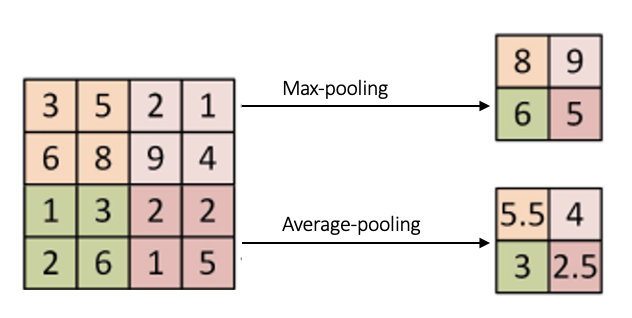
\includegraphics[width=0.8\linewidth]{max.png}
\caption{Example of pooling operations. The kernel size is 2×2 and the stride is 2 pixels.}
\label{ma}
\end{figure} 
Figure~\ref{p1} demonstrates that the layer units are correlated to three spatially adjacent units in layer m-1. Also, in CNN, all convolutional filter is duplicated over the whole layer, receiving the same weights and biases. In Figure~\ref{p2}, the weights of the equivalent color are compelled to be identical. In this way, CNNs can accomplish more useful generalizations on computer vision problems. The training performance is enhanced by significantly decreasing the number of unconstrained parameters to be determined. The input and output of individual layers are collections of arrays named feature maps. A conventional CNN regularly comprises three essential layers: (I) a convolutional layer, (II) nonlinear layer, and (III) pooling layer.
\begin{figure}[H]
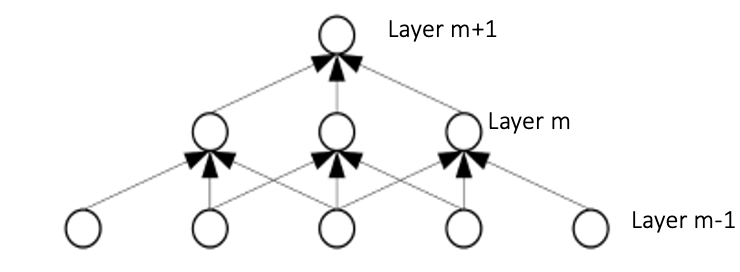
\includegraphics[width=0.8\linewidth]{poo.png}
\caption{Local connectivity design in CNNs. Every unit is correlated to three spatially adjacent units in the layer below [64]}
\label{p1}
\end{figure} 
\begin{figure}[H]
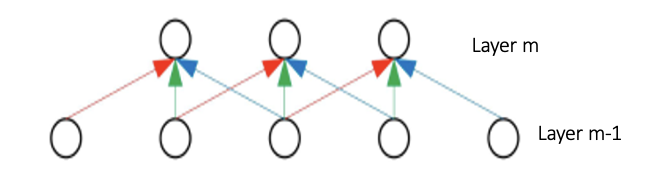
\includegraphics[width=0.8\linewidth]{play.png}
\caption{Shared weights in CNNs. The identical color symbolizes the equivalent weight.}
\label{p2}
\end{figure} 
The activation function embedded in the nonlinear layer is applied to each feature map to learn nonlinear descriptions. The rectified linear unit (ReLU) is the most extensively utilized activation function in recent deep neural networks. It is mathematically represented as: $f(x) =max(0,x)$. In other words, ReLU outsets the non-positive value as zero and keeps the positive value unchanged. ReLU can mitigate the vanishing gradient intricacies whiles expediting the learning process to obtain a significant decline in training time. \par
In recent years, CNN's breakthrough in object detection, recognition, and similar tasks has driven researchers to investigate their capacity to directly learn a non-linear mapping between a hazy input image and its identical transmission map\citing{a45,a46,nw1,80}. Tang\citing{a47} orderly study various haze-relevant features in a learning structure with random forest\citing{a48} to recognise the most suitable feature combination for haze removal. In Zhu\citing{a49}, a linear model depending on a colour attenuation prior is adopted to predict a hazy image's object scene depth through a supervised-learning method. Notwithstanding the exceptional results, haze-relevant features are not sufficiently compelling. Cai et al.\citing{a50} proposed a trainable end-to-end network for estimating the transmission map. DehazeNet produces excellent visual effects on real images compared to traditional methods. However, spatial variability in hazy vision complicates learning the relationship between the input image's haze transmission and spectral-spatial information. In\citing{a51}, results are achieved from training a multi-layer perceptron to compute Image deconvolution. Xie et al.\citing{a52} address multiple types of noise and in-painting that the dehazed image has by using stack sparse denoising Auto-encoders (SSDA). Ren et al.\citing{a53} determines the transmission map by learning the connection between the distorted image and their corresponding propagation map. The propagation map is finally refined with a coarse-scale and fine-scale network. Dudhane et al.\citing{a54} solved colour deformity problem derived from an inaccurate estimation of the transmission map using multi-stage CNN. First, a multi-channel depth map is derived from the network to learn the hazy image's colour information. Finally, the transmission map is estimated from the multi-channel. He\citing{a55} designed an end-to-end network(DCPDN) which jointly estimates the transmission map and atmospheric light using the degradation model. Finally, edge-preserving methods are applied to the final output to reduce halos. In\citing{a56}, an encoder-decoder network is used in dehazing a single Image while preserving the edges of the output image. Qin et al.\citing{a57} proposed a feature fusion attention end-to-end network. The network maintains a certain percentage of information, which is later transferred to estimate and retrieve a haze image. Extensive experimental results illustrate that CNN's use in image restoration problems is more efficient and robust than traditional algorithms that depend on strong assumption or priors. Boys\citing{a58} proposed the novel Aod-net, end-to-end architecture for haze removal. Compared to all other deep learning methods, the Aod-net is very simple. Primarily this network adopts a simplistic approach to estimates the atmospheric light and transmission map. Li\citing{a59} solved the haze removal problem by adopting an encoder and decoder architecture using a conditional generative adversarial network (cGAN). In this model, an end-to-end trainable neural network predicts the transmission map to obtain a haze free image. Jiang\citing{a60} adopted a multi-scale residual convolutional neural network (MRCNN) to achieve dehazing for remote sensing images. To estimate the transmission map, they employ a 3D convolutional kernels to obtain spatial spectral relationship information and conceptual features from surrounding pixels. 
\section{Image Contrast Enhancement Method}
The principal aim of contrast enhancement algorithms is to enhance the contrast of the image. The approach is extensively utilized in image dehazing and underwater image enhancement. This thesis classifies the image contrast enhancement method into two: (I) Retinex based and (II) contrast enhancement. 

\subsection{Retinex-based}
Retinex originates from two words, "retina" and "cortex," meaning biological optical viewpoint. The Retinex algorithm's purpose for image enhancement is to achieve effective range compression and color consistency concurrently\citing{4,5,6}. Edwin\citing{a61} originally proposed the Retinex approach based on the color resolution. The Retinex theory has since widely been adopted in image dehazing\citing{a62,a63,a64}. The theory assumes that an image comprises of two components: (I) a reflection component, which is the inner information of an image, and (II) an incident component, which represents the luminance of an image. Early research focused on estimating iteration methods, the luminance of an image, and a multiple-scale algorithm based on the difference-of-Gaussian (DOG) filter\citing{a65}. The multi scale Retinex (MSR) algorithm and the multi scale Retinex with color restoration (MSRCR)
algorithm were proposed to address the shortcomings of SSR \citing{a66,a67,a68}. Jobson\citing{a69} proposed the original single scale Retinex (SSR) algorithm using the Gaussian function to estimate an image's luminance. However, the SSR cannot concurrently perform effective range compression and color performance. Originally Hu\citing{a70} applied the bilateral filter to calculate the image's luminance and further applied the Gamma adjustment and sigmoid function to intensify the image's reflection. The novel variable filter Retinex algorithm proposed by Yang\citing{a71} adapt the scale parameters for each hazy image's local region. The proposed algorithm significantly amplifies the local contrast of the image while increasing clarity. 

\begin{table}[!htb]
    \centering
    \caption{Comparison of image dehazing algorithms using Figure~\ref{fig4}.}
    \begin{tabular}{ | m{2.5cm} | m{4.5cm}| m{4.5cm} | m{2.8cm} | } 
        \hline
        \textbf{Method} & \textbf{Advantages} & \textbf{Disadvantages} & \textbf{Application} \\
        \hline
        Multi-Image Method & 
        \begin{itemize} 
            \item Dehazed image has excellent color fidelity. 
            \item Final haze free image contains Small halo effect.
            \item High image visibility under thin haze. 
        \end{itemize} & 
        \begin{itemize} 
            \item It is challenging to obtain images of different scenes
            \item Fail to restore images with high haze density.
        \end{itemize} & A unique application such as surveillance.
        \\
        \hline
        Single-Image Method & 
        \begin{itemize} 
            \item Suitable for hazy night time and daytime images. 
            \item Final haze free image contains Small halo effect.
            \item Final haze free image has little halo effect
            \item Dehazed image has excellent color restoration. 
        \end{itemize} & 
        \begin{itemize} 
            \item The adoption of a strong prior creates high computational cost.
            \item Fail to restore images when the sky region is white.
        \end{itemize} & Single color or grayscale image.
        \\
        \hline
        Retinex-based & 
        \begin{itemize} 
            \item Computational cost is very low. 
            \item Simple method but very robust.
            \item Suitable for images with low intensity
        \end{itemize} & 

        \begin{itemize} 
            \item Fail to dehaze images with high haze density.
            \item Cannot enhance local information of the hazy image. 
        \end{itemize} & Single color or grayscale image.
        \\
        \hline
        Contrast enhancement & 
        \begin{itemize} 
            \item The resultant image has High contrast. 
            \item Final haze free image contains less noise. 
            \item Good edge preservation
        \end{itemize} & 

        \begin{itemize} 
            \item Unable to dehaze images with high haze density.
            \item Final haze free image has little halo effect. 
        \end{itemize} & Single color or grayscale image.
        \\
        \hline
        Fusion-based & 
        \begin{itemize} 
            \item The resultant image visually appealing.
            \item Dehazed image has great contrast. 
        \end{itemize} & 

        \begin{itemize} 
            \item High computational cost with low efficiency.
            \item Highly complex 
        \end{itemize} & Single color or grayscale image.
        \\
        \hline
    \end{tabular}
    \label{Tab1}
\end{table} 



\subsection{Contrast Enhancement method.} 
An image histogram is a kind of histogram which offers a graphical representation of the tonal appropriation of the gray qualities in a computerized picture\citing{7,8,9,10}. By review the image's histogram, we can examine the frequency of appearance of the changed gray levels contained in the image. Histogram equalization is a technique that constructs a gray map which alters the histogram of image and reconstructs all pixel values to produce desire histogram results specified by user\citing{a71}. The gray level of the image is transformed, based on the probability distribution of the input gray levels. That is it provides a statistical probability distribution of each gray level of an image. This method improves the contrast in an image, in order to stretch out the intensity range. HE is the most common method used due to its austerity and the degree at which it produces desired result. Disadvantages of HE includes: (I) The Histogram Equalization method does not take the mean brightness of an image into account. (II) The HE method may result in over enhancement and saturation artifacts due to the stretching of the gray levels over the full gray level range. (III) Nevertheless, HE is not commonly used in consumer electronics such as TV because it may significantly change the brightness of an input image and cause undesirable artifacts. (IV) If there are gray values that are physically far apart from each other in the image, then this method fails\citing{a74}. 

\begin{figure}[!htb]
	\centering
	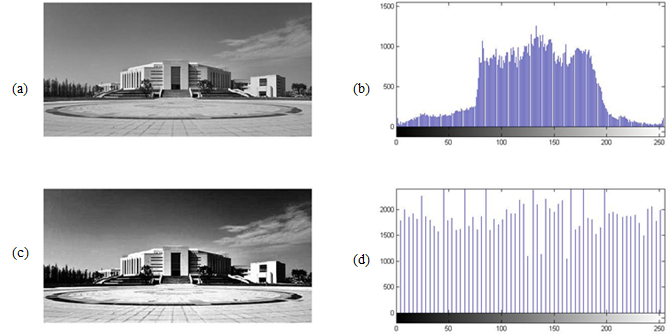
\includegraphics[width=5.6in]{Picture1.png}
	\caption{(a) Original frame of low quality. (b) HE enhancement result. (b) Histogram of original image. (d) Histogram of enhanced image}
	\label{11}
\end{figure}
This thesis categorizes Histogram equalization into two methods: global and local histogram equalization. Global histogram equalization (GHE) applies the whole input image histogram information as to its transformation function. GHE is excellent for comprehensive enhancement. However, this method ignores the brightness of the input image during enhancement. GHE restricts contrast, therefore resulting in contrast loss for grey levels having weaker frequencies. To address, the drawbacks local histogram adjustment (LHE) techniques have been proposed. It utilizes a little window that slides through each pixel of the input image consecutively.  In this way, it presents the utilization of nearby information. LHE demands a substantial computational cost and sometimes creates an over enhancement in some parts of the image. Also, this approach can magnify the noises in the input image beside the image highlights. The high computational expense of LHE can be minimized using non-covering piece based HE. GHE cannot ensure adequate variation upgrade in all regions of the image. On the other hand, LHE captures the definite details of its input image adequately; however, it also generates noise. Histogram equalization, typical histogram specification, and gamma amendment to enhance global complexity appearance only extend the intensity's global dispersion. More varied models are demanded to subdue such downside. Tobergte et al.\citing{c7} adopts a varied filter that measures the honing way commitment so that differentiation improvement happens in particular high areas and small or no image honing happens in smooth zones. Saenko et al.\citing{c8} employs two versatile histogram balance methods to modify power dissipation inside small regions. Histogram equalization is a straightforward and compelling complexity upgrade method that carries pixel values consistently such that an enhanced image has a directly combined histogram and is a global operation. Hence, it does not save the image intensity. 
Numerous  HE-based procedures have been proposed to address the drawbacks of traditional Histogram equalization. The Bi-histogram equalization (BBHE) approach separates the histogram into two sub-histograms because of different partitioning converges. Next, every sub-histogram is evened out completely, taking into account the histogram balance. These procedures can defend image illumination more when opposed to the Histogram Equalization. The (BBHE) algorithm proposed by Kim et al.\citing{c9} utilizes independent histogram equalization individually over two sub-images achieved by decomposing the input image based on its mean with a constraint that the resulting equalized sub-images are bounded by each other the input means. Like (BBHE), Wang et al.\citing{c10} proposed Dualistic Sub-Image Histogram Equalization (DSIHE). This novel histogram equalization method divides the first image is into two equal range sub-images given its dark level thickness range. At that point, the two sub-images are evened out individually. Finally, we get the outcome after the prepared sub-images are made into one image.  The calculation can enhance the visual image data viably and compel the first image's average luminance from excellent movement. This makes it conceivable to be used in a video framework straightforwardly. However, these techniques utilized median value rather than mean to isolate the info histogram and demonstrated preferred brightness preserving over BBHE and Histogram Equalization\citing{c11}. DSIHE is the best method for preserving the first image brilliance. Furthermore, it improves the image data successfully. BBHE and DSIHE are limitedly suitable for images demanding a higher level of brilliance protection to refrain from irritating ancient rarities.
 Minimum Mean Brightness Error Bi-Histogram Equalization (MMBEBHE) was proposed by Chen et al\citing{c12}. This approach is an augmentation of BBHE, which allows maximum illumination safety. MMBEBHE method separate histogram into two sub-parts using a threshold level, yielding the least Absolute Mean Brightness Error (AMBE). A definitive objective behind this procedure is to authorize the most significant level of brightness conservation in Bi-Histogram Equalization to stay away from offensive relics and unnatural upgrade because of inordinate balance, furthermore to detail a productive, recursive and number based answer for surmised the yield means as an element of a limit level. Mimicked results from MMBEBHE shows that it has safeguarded better splendour and yielded a more normal upgrade\citing{c13,c14}. BBHE and MMBEBHE have superior conservation and improvement levels contrasted with HE and DSIHE\citing{c15,c16}
Jin et al.\citing{c17} introduced the Range Limited Bi-Histogram Equalization (RLBHE). This approach separates the input histogram into two independent sub-histograms by a threshold that minimizes the intra-class variance. This was carried out to separate the objects from the background effectively. This method visually presents a more pleasant contrast enhancement while sustaining the input brightness, and it is simple to implement in real-time processing. This thesis has chosen some conventional image and apply HE, BBHE, DSIHE, and MMBEBHE methods to assess their appearance. Figure~\ref{11} shows the experimental results

\begin{figure}[H]
	\centering
	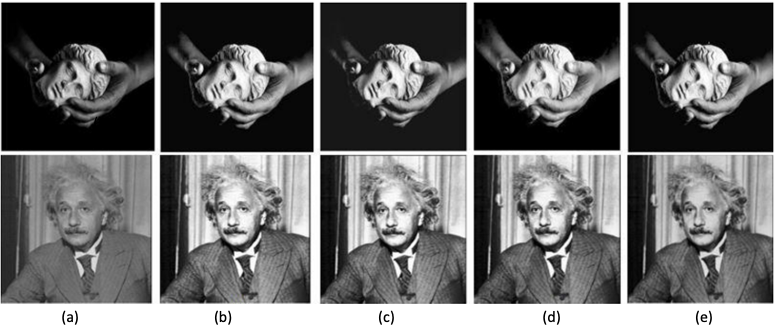
\includegraphics[width=5.5in]{Picture2.png}
	\caption{(a) Input image (b) HE method (c) BBHE method (d) DSIHE method (e) MMBEBHE method}
	\label{fig89}
\end{figure}

The histogram of a hazy image usually is distributed since the majority of pixels are gray-scale as shown in  Figure~\ref{11}. The intensity transformation of hazy images is effective due to its enhancement of the image's histogram. In contrast enhancement, the most common algorithms used are power-law gamma transformation, piecewise-linear transformation, and histogram equalization (HE). These algorithms improve the brightness of the final haze free image. Histogram equalization expands the dynamic range of the hazy input image by redistributing its histogram. In this dissertation, we group Histogram equalization into global histogram equalization (GHE) and local histogram equalization (LHE)\citing{a71,a72}. Global histogram equalization (GHE) was first adopted to enhance the hazy image whiles reducing halos with wavelet transformation\citing{a73,a74}. Ma\citing{a75} utilized a piecewise-linear transformation to enhance further the SSR algorithm discernibility algorithm. To decrease noise produced by the histogram equalization algorithm, contrast limited adaptive histogram equalization (CLAHE) has been adopted by many researchers\citing{a76,a77}. Even though contrast enhancement reduces the amount of haze, the final image appears unrealistic due to the direct manipulation of each RGB color channel\citing{a78,a79}. However, this method achieves better results compared to Retinex-based methods. 
\begin{table}
    \centering
    \caption{Comparison of image dehazing algorithms using Figure~\ref{fig4}.}
    \begin{tabular}{ | m{2.9cm} | m{1.8cm}| m{4.6cm} | m{3cm} | } 
        \hline
        \textbf{Fusion Algorithm}& \textbf{Domain} & \textbf{Advantages} & \textbf{Disadvantages}  \\
        \hline
        Discrete wavelet transforms (DWT)& 
        Transform & 
        \begin{itemize} 
            \item The DWT union procedure may overcome the maligned fusion strategy as far as restricting the unearthly bending.
            \item It further presents a more reliable signal to noise ratio compared to the pixel-based method. 
        \end{itemize} & In this method, the ultimate fused image has a limited spatial resolution. 
        \\
        \hline
        
        Combine Discrete wavelet transforms & 
        Transform & 
        \begin{itemize} 
            \item Multi-level fusion, where the image experiences fusion twice using an efficient fusion technique, presents an enhanced outcome. 

            \item Output image includes both high spatial resolutions with high-quality spectral content. 

        \end{itemize} & This method is complicated in the fusion algorithm. Demands an excellent fusion algorithm for a more reliable result. 


        \\
        \hline
        Simple Average & Spatial & 
        This is the simplest method of image fusion & The principal limitation of the Pixel level method is that this method does not provide a guarantee to have an accurate image from the set of images 
        \\
        \hline
    \end{tabular}
    \label{Tt}
\end{table} 
\subsection{Fusion based} 
Image fusion is a procedure of consolidating the applicable data from an image arrangement into a single image, where the resultant intertwined image will be more useful and finish than any of the information images. Image fusion systems can enhance the quality and increment the use of this information. Fusion algorithms can be classified into low, mid, and high levels. 
In some literature, this is alluded to as a pixel, feature, and symbolic levels. In the image fusion procedure, each given image's critical data are melded to shape a resultant image whose quality is better than any of the info Images. Image combination technique can be extensively characterized into :(I) Spatial domain fusion method (II) Transform domain fusion. In spatial domain strategies, we straightforwardly manage the image pixels. The pixel qualities are controlled to accomplish the fancied outcome. In recurrence space strategies, the image is initially moved into the recurrence area. It implies that the Fourier Transform of the image is figured first. All the Fusion operations are performed on the Fourier change of the image, and afterwards, the Inverse Fourier change is performed to get the resultant image. Image Fusion connected in each field where the image is should be investigated\citing{g1,g2,c3,c4}. For example, medical image analysis, microscopic imaging, examining images from satellite, remote detecting Application and PC vision. The fusion methods such as averaging, proven method, principal component analysis (PCA) and IHS based methods fall under spatial domain approaches
 Another vital area in the spatial domain fusion method is the high pass filtering based technique. The drawback of spatial domain approaches is that they create spatial distortion in the melded image. Spectral distortion becomes a negative factor while we go for further processing, such as a classification problem. The discrete wavelet change has turned into a precious tool for fusion. Some other combination techniques are additionally there, for example, Laplacian pyramid based, Curvelet transform-based\citing{c5,c6,g3,g4,g5}. These strategies demonstrate a superior execution in the melded image's spatial and spectral nature contrasted with other spatial techniques for fusion. Different techniques have been created to perform image fusion\citing{c18,c19,c20,c21,c22,c23,c24}. Some outstanding image fusion strategies are 
\begin{enumerate}
\item  Wavelet transforms: (i) Discrete wavelet transforms (DWT) (ii) Stationary wavelet transforms (iii) Multi wavelet transforms. 
\item Pyramid method: (i) Gaussian pyramid (ii) Laplacian Pyramid (iii) Gradient pyramid (iv) Morphological pyramid.
\item Intensity hue saturation (IHS) transform based fusion.
\item  Principal component analysis (PCA) based fusion
\end{enumerate}
To further precisely present image enhancement based on fusion, we briefly review the existing image fusions algorithm and its advantages. Table~\ref{Tt} shows a brief survey of the image fusion algorithm. 
 \section{Summary}
 This chapter presented an in-depth detailed analysis of haze removal algorithms with their advantages, disadvantages, and application. Although single image dehazing algorithms have received significant development in past years, there are still many problems which need to be addressed. The main problems are as follows:
\begin{itemize} 
            \item A small number of technologies can ascertain whether the existing object scene carries haze or not. The current haze removal algorithms only can restore a hazy image. So, it is essential to overcome this problem in the future.
            \item There is no single image dehazing algorithm that can achieve reliable performance in all varieties of hazy climate conditions. Existing single image dehazing algorithms can efficiently intensify an image with uniform haze or a low, dense, hazy image.
            \item The haze degradation model may not be the excellent model for different scenes, such as on the sea or air. So, it is essential to discover a more suitable model or multiple designs for numerous scenes. Furthermore, the parameters used in these models can expressly be set in terms of the haze level of images.
        \end{itemize}

\chapter{A Fast Single-Image Dehazing Using DCP and Rayleigh Scattering}\label{Chapter:Ch3}
This chapter proposes a novel fast single image dehazing method based on dark channel prior and Rayleigh scattering. Outdoor images are affected by natural and artificial adverse weather conditions such as mist, smoke, haze, fog, and smog due to the discernibility diminishing aerosols, which substantially cause a color change, image degradation, and scene darkening, among others. These aerosols are the arrangement of solid or fluid particles suspended by a blend of gases\citing{h1,h2,h3,h4,h5}. The presence of sunlight, high relative humidity, and stagnant airflow enhance the reactions that lead to the formation of aerosols\citing{a5}. Image dehazing has two aims\citing{a23,a24,d6}: (1) improving the visibility scene and correct the loss of light intensity caused by apparent aerosols, and (2) improving consumer photography and computer vision application. However, dehazing is a significant problem in computer vision and image processing due to its dependence on unknown scene depth\citing{d1,d2,d3,d4}. 
In this dissertation, we adopt the theory of dark channel prior and Rayleigh scattering to reduce computational time whiles achieving high-quality dehazed images. Firstly, we present a simple but effective methodology for estimating the atmospheric light by computing average, minimum, and maximum pixels in each of the three color channels. Utilizing the theory of Rayleigh scattering, we estimate a scattering coefficient to calculate the initial transmission map. A fast guided filter is further utilized to improve the estimated transmission map due to incorrect halo edges. Ultimately, we retrieve the haze-free image using the atmospheric scattering model. In this respect, the method proposed in this dissertation is at most two orders of magnitude faster than most conventional dehazing algorithms. Furthermore, collected qualitative and quantitative outcomes utilizing apparent edge contrast prove that the proposed method produces more reliable results than another recently introduced state-of-the-art algorithm. The rest of the chapters are organized as follows. In Section~\ref{bk}, there is an overview of the theoretical foundation used in this dissertation. Section~\ref{bc} describes the proposed algorithm and its implementation. Section~\ref{be} shows experimental results and, Section~\ref{con} concludes this work.

\section{Background} \label{bk} 
This section presents concepts such as dark channel prior and Rayleigh scattering used for the proposed technique for single image dehazing. 

\subsection{Rayleigh Scattering}
Rayleigh scattering happens when light combines with particles in the atmosphere that are more diminutive in diameter than the incoming light wavelength. The distribution defines the change of the intensity of scattered light with direction. The dispersion is fundamentally due to oxygen and nitrogen molecules\citing{a80,a81,a82}. This method additionally predicts the polarization of the scattered light. These molecules receive the light and re-transmit it arbitrarily. The wavelength of light is depicted in a spectrum of different colors from 400 nm at violet to 700 nm at the red end with orange, yellow, green, blue, and indigo in the middle\citing{a83}. On the visible spectrum, blue light has a tremendous frequency and a smaller wavelength than red light. Atmospheric particles scatter the original light $I_o$ in a specific direction $\theta$\citing{a84}. The model is formulated mathematically as:
\begin{equation}\label{rayleigh}
	I=I_0 S(\lambda,\theta,d)
\end{equation}
where:
\begin{equation}\label{rayleigh1}
	s(\lambda,\theta,d)=\frac{\pi^2(n^2-1)^2}{2} \frac{\rho(d)}{N} \frac{1}{\lambda ^4} (1+cos^2\theta)
\end{equation}
The wavelength of the incoming light is represented by $\lambda$  at an angle $\theta$. $n$ and $N$ are the refractive index of air and atmospheric density, respectively. Depending on the incoming light, various angles receive more light. We observe that the amount of light scattered depends on the wavelength of the incoming light. Thus, as air passes through all the colors on the visible spectrum, blue light scatters more than green and red light. The scattering level depends on how quickly charged particles oscillate. The intensity of scattered light is proportionate to the fourth power.

\begin{figure}[H]
	\centering
	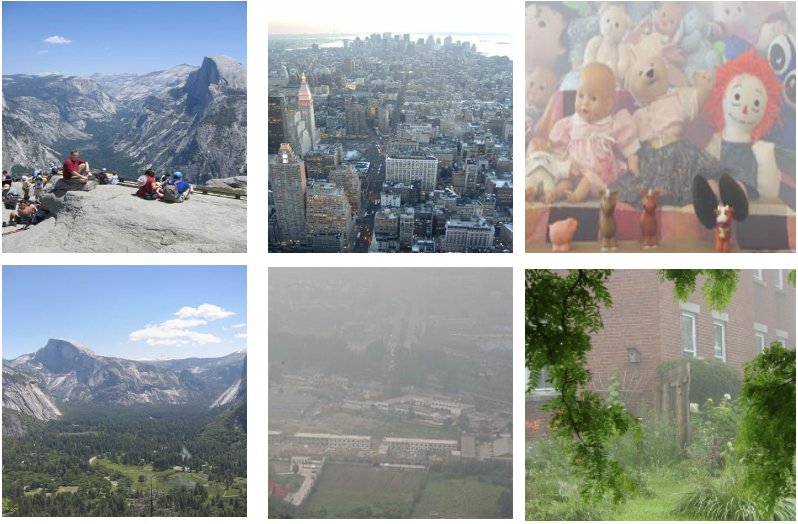
\includegraphics[width=5.6in]{sa.png}
	\caption{Sample Hazy Images}
	\label{figsa}
\end{figure}

\subsection{Dark Channel Prior}
Inspired by an earlier haze elimination algorithm known as dark object subtraction\citing{a85}, the dark channel prior relies on empirical observation of haze free images attributes. A prior is a theory or knowledge built previously. He et al.\citing{a33} proposed that some pixels whose intensity is very low in an arbitrary image patch and approaches 0 in at least one color channel for outdoor haze free images. These dark pixels are associated with shadows of the object (trees, buildings, and cars)\citing{d7,d8,d9,d10}, dark entities, and items that are principally a blend RGB color channels, as shown in Figure~\ref{fig10}. It is meriting to state that the dark channel is an operation on an image, whether the image contains haze or not. In light of this statistic, for a haze free image $I$, its dark channel can be expressed mathematically as a minimum value operation in patches around the target pixel:  
\begin{equation}
	I^{dark}(x)=\min_{c\in(r,g,b)} \bigg(\min_{y\in\Omega(x)}(I^c(y))\bigg)
\end{equation}
where $I^c$ represents intensity of the color channels ${(r,b,g) \in c}$. $\Omega(x)$ is a rectangular patch centered at pixel $(x,y)$. When we apply the observation to a haze free image, we obtain:
\begin{equation}
	I^{dark}(x) \rightarrow 0
\end{equation}
Note individual pixel in $I^{dark}$ is a scalar. A dark channel is the result of the two least operators. The operator $\min_{c\epsilon(r,g,b)}$ is performed on each pixel. It is meriting stating that the dark channel is an operation on an image, regardless of the image's nature (hazy or haze free). We can similarly calculate the dark channel $I^{dark}(x)$ of a hazy image $J$ as: 
\begin{equation}
	I^{dark}(x)=\min_{c\in(r,g,b)} \bigg(\min_{y\in\Omega(x)}(J^c(y))\bigg)
\end{equation}

Even though the algorithm produces superior results, it has some shortcomings: (1) high computational time due to soft matting, and (2) the algorithm can not produce quality outcomes when the object scene is relative to the atmospheric light. 

\begin{figure}[H]
	\centering
	\includegraphics[width=5.7in]{10.png}
	\caption{Dark channels of arbitrary haze free images. We compute the least of $(r, g, b)$ values for individual pixel with the patch size of 15x15}
	\label{fig10}
\end{figure}
\section{Contribution} \label{bc}
The transmission map and atmospheric light have essential functions in haze removal. Therefore, an excellent dehazing algorithm with a calculation of both the transmission map and the atmospheric light can process a hazy image's restoration competently. Haze, which is generated by atmospheric attenuation, relies on the number of particles in the atmosphere. According to the haze degradation model, both the transmission map and the atmospheric light remain relevant portions. Thus, the transmission map and atmospheric light must be enhanced. This chapter proposes a novel methodology for single image dehazing based on the DCP theory\citing{a33}.The method comprises three steps (Figure~\ref{fig11}): (I) estimation of transmission map $t$; (II) atmospheric light $A$; and (III) recovery of the scene radiance.
\begin{figure}[H]
	\centering
	\includegraphics[width=4.6in]{100.png}
	\caption{Statistics of the dark channels. (a) Distribution of the pixel intensity of all of the 5,000 dark channels (each bin represents 16 intensity levels). (b) Cumulative distribution. (c) Distribution of the average intensity of each dark channel.}
	\label{fig10}
\end{figure}
The proposed method employs Rayleigh scattering to estimate the scattering coefficient used in calculating the transmission map $t$. The principal challenge retrieving $J$ from the haze degradation model are the unknown parameters, $A$ and $t$. The number of image pixels is equivalent to the cumulative number of unknowns. Therefore, the utilization of priors and assumptions in estimating $t$ and $A$ to retrieve $J$ is imperative. The traditional algorithm, which depends on the dark channel prior, makes it conceivable to lead a precise estimation of $A$ and $t$, yet at a higher computational time.
\begin{figure}[H]
	\centering
	\includegraphics[width=5.3in]{11.png}
	\caption{Framework of the proposed image-dehazing algorithm}
	\label{fig11}
\end{figure}
\subsection{Atmospheric Estimation}
 A critical element in solving the hazy imaging model is the estimation of $A$ \citing{z1,z2,z3,m1}. To obtain the transmission map $t$, we first estimate the atmospheric light $A$. The atmospheric light portion must be correctly decided for an efficient haze removal algorithm. An inaccurately determined atmospheric light will produce abysmal dehazing results.
 Numerous traditional DCP-based dehazing methods calculate the atmospheric light by choosing the pixel with the most considerable dark channel value as follows \citing{a86,a87,a88,a89,a90,z4}:
\begin{equation}
A=I(argmax_x(I^{dark} x))
\end{equation} 
However, the above approach can inaccurately choose the pixel when the scene comprises colourful items\citing{a88,a89,a90,a91}. Based on the high correlation between the density of haze and the dark channel pixel value a large number of algorithms, we first select the top $p\%$ of the brightest pixels in the dark channel, followed by the selection of the color with the highest intensity value among the selected pixels to estimate $A$. However, illuminated objects ( white cars and buildings) appearance generates an incorrect estimation. 
Therefore, to calculate the pixel with accurate luminance representation of the haze density, we propose an algorithm where both the brightest and darkest pixels are computed. The main steps are as follows:\par
\textbf{Step 1:} According to the theory of Rayleigh scattering, blue light scatters the most on the colour spectrum because it progresses as shorter, smaller waves. The pixels in this channel are frequently in the complex region.  This is due to mainly atmospheric lights that access the imaging channel. We reduce the block effect by choosing pixels with an immense intensity in the input image's blue channel. The maximum pixel selected from this channel accounts for the brightest part of the image. Experimental outcomes prove that the method eliminates the salt-and-pepper noise generated by the white objects and further improves $t$.
\begin{equation}
A_1= \max_{ij}x(I_B)
\end{equation} 
\textbf{Step 2:} In the second step, we compute the lowest pixel's average in the red and green channel of the input image. This step considerably eliminates undesired texture information from $A_1$. 
\begin{equation}
A_2= \arg\min_{ij}x(I_G,I_R)
\end{equation} 
\textbf{Step 3:} Finally, we calculate the atmospheric light $A$ by the aggregate of $A_1$ and $A_2$. 
\begin{equation}
A= (\arg\min_{ij}x(I_G,I_R))+(\max_{ij}x(I_B))
\end{equation} 

\begin{figure}[H]
	\centering
	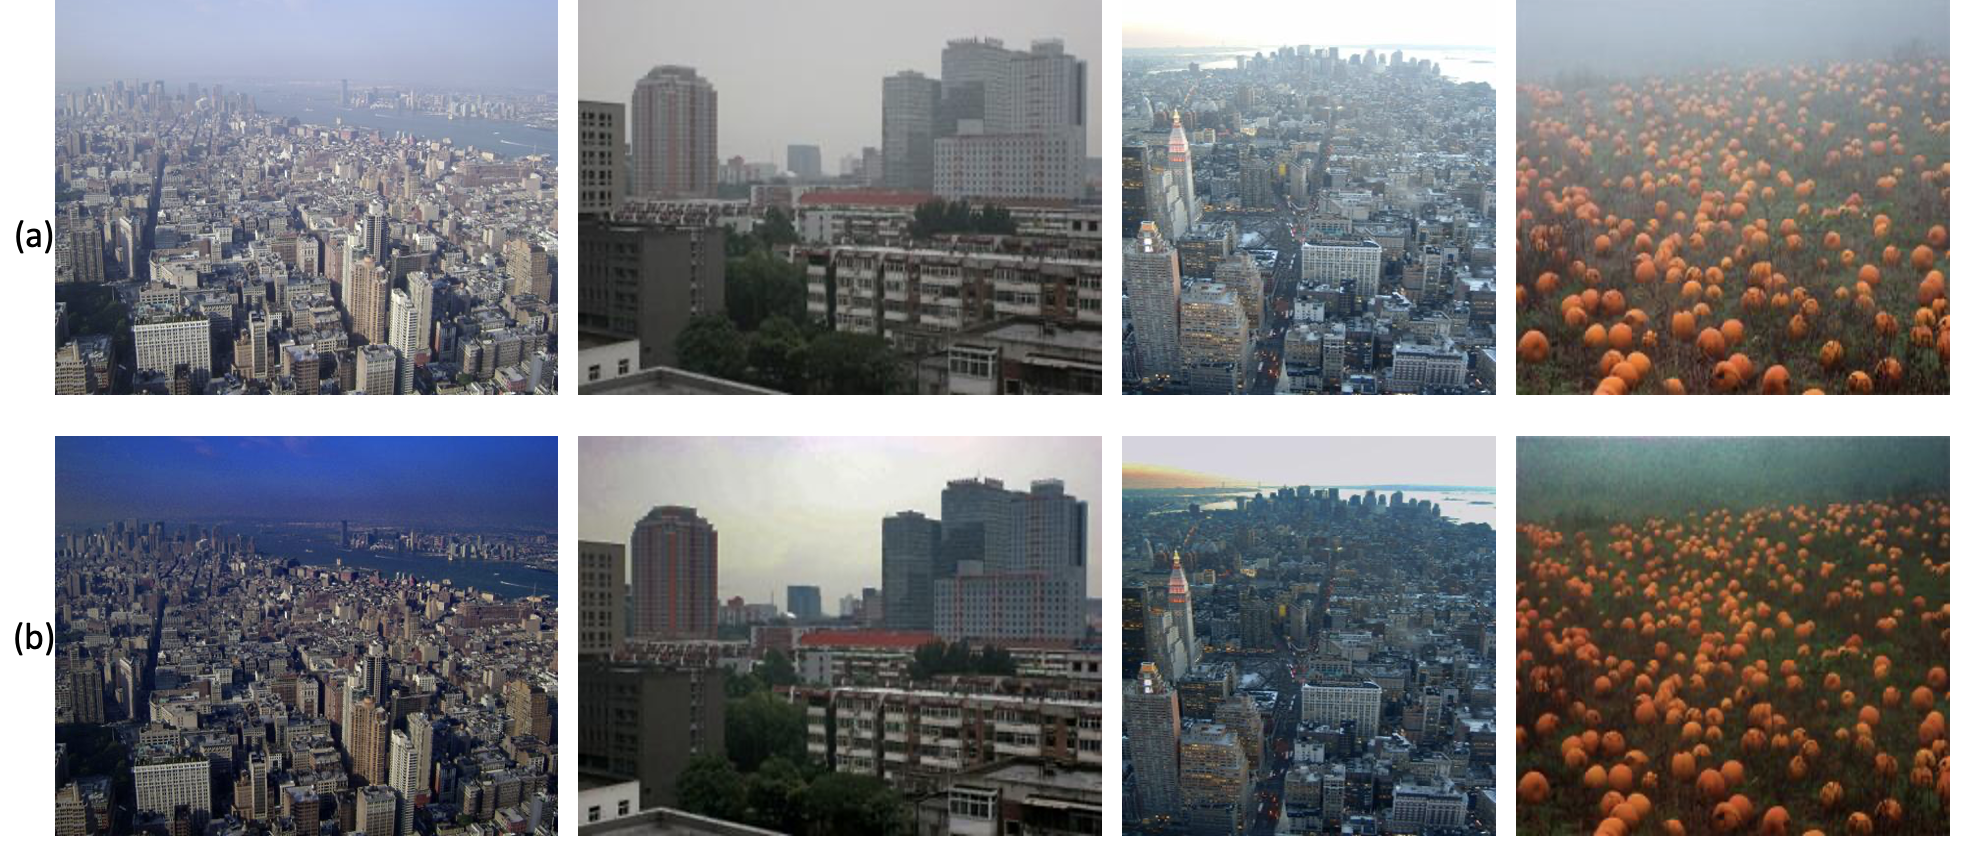
\includegraphics[width=1.0\linewidth]{sample.png}
	\caption{Sample dehazing result using our method. (a) Input Hazy image (b) Dehazed Image}
	\label{s}
\end{figure}
\subsection{Transmission map estimation}
The transmission map's prediction from a provided input hazy image is considered a pixel-level image regression task.
Another significant part of solving the haze imaging equation is the accurate estimation of $t(x)$. Transmission map, $t(x)$ is the portion of the light that reaches an observer without scattering. Inaccurate estimation of $t(x)$ can formulate false textures, blocking artefacts and high computational consumption. In a uniform climate, a scattering coefficient $\beta$ forms part of the transmission $t(x)$. Unfortunately, such a model is only accurate for small images and eliminates or accommodates the directional parts of atmospheric interference. The drawback of DCP is the inaccurate calculation of $t$, which adds a high computational time. We calculate the fraction of light intensity loss in all directions using Equation~\ref{rayleigh} to address this problem. We first compute the derivative of light energy dispersed in all directions.

\begin{equation}\label{1}
\beta(\lambda)=\int\limits_0^{2\pi} \int\limits_0^\pi s(\lambda,\theta,d) \sin{\theta} d\theta d\phi
\end{equation}
where $ \beta(\lambda)$ is the fraction of light lost after a single atmospheric scattering. We rewrite Equation~\ref{1} by expanding the constant terms $s(\lambda,\theta,d)$ with Equation~\ref{rayleigh} to determine values that depend on $\theta$.
\begin{equation}\label{elimination}
\beta(\lambda)=\int\limits_0^{2\pi} \int\limits_0^\pi \frac{\pi^2(n^2-1)^2}{2} \frac{\rho(d)}{N} \frac{1}{\lambda ^4} (1+cos^2\theta)\sin{\theta} d\theta d\phi \end{equation}
Equation~\ref{elimination} is simplified by moving all the constant terms $s(\lambda,\theta,d)$.
\begin{equation}\label{constant}
\beta(\lambda)= \frac{\pi^2(n^2-1)^2}{2} \frac{\rho(d)}{N} \frac{1}{\lambda ^4}\int\limits_0^{2\pi} \int\limits_0^\pi (1+cos^2\theta)\sin{\theta} d\theta d\phi \end{equation}
This new equation provides one more approach to see how various colors of light are scattered. To determine the ratio of light that is lost to scattering after a single collision, we find the outer integration of Equation~\ref{constant}:
\begin{equation}\label{inner}
\beta(\lambda)= \frac{\pi^2(n^2-1)^2}{2} \frac{\rho(d)}{N} \frac{1}{\lambda ^4}\int\limits_0^{2\pi} \frac{16\pi}{3} d\phi \end{equation}
\begin{equation}\label{inner}
\beta(\lambda)= \frac{8\pi^2(n^2-1)^2}{3} \frac{\rho(d)}{N} \frac{1}{\lambda ^4} \end{equation}
\begin{figure}[H]
	\centering
	\includegraphics[width=1.0\linewidth]{12.png}
	\caption{Comparison of $t$ before and after refinement using images from Figure~\ref{figsa}.(a) Refined Transmission map $t$ (b)Transmission map}
	\label{fig12}
\end{figure}

The transmission map depends on three main factors: (I) scattering coefficient $\beta$  (II) scene depth $d$ and (III) atmospheric light $A$. From Equation~\ref{inner} and a prior $A$, we estimate initial $t^1$ as follows:
\begin{equation}
	t^1(x)=\frac{\beta(\lambda)d}{A} 
\end{equation}
where $A$ is the atmospheric light, $d$ is the scene depth, and $\beta$ is the scattering coefficient. Outdoor hazy images contain a bright section and may affect $t$. To deal with this, we compute the maximum average of the three RGB color channels and compare the value to $t^1$. If the resultant value is greater than $t^1$, then this region is seen as bright. Otherwise, we considered this region as non-bright. To address the bright region, we introduce a directional component $(1+cos^2\theta)$ where $\theta$ represents the angle between the object scene and the camera. The corrected transmission map improves bright areas without color distortion. 
In practice, removing the entire haze from an image results in the image lacking a sense of depth. In this regard, we introduce a correction factor $\omega(0<\omega\leq 1)$ to retain a small amount of haze. In this study, we set $\omega$ to 0.95. The final transmission $t$ map is estimated as follow:
\begin{equation}
t(x)= 1-\omega \frac{\beta(1+cos^2\theta)d}{A} 
\end{equation}

\begin{figure}[H]
	\centering
	\includegraphics[width=1.0\linewidth]{13.png}
	\caption{Comparison of depth estimates. (a) Input Hazy image (b) estimated transmission map. (b1) He [56] (b2) Our method (c) Refined transmission map. (c1) He [56] (c2) Our method (d) Dehazed image (d1) He [56] (d2) Our method.
}
	\label{fig13}
\end{figure}


\subsection{Transmission map refinement} 
The inaccurate calculation for the transmission map can lead to some difficulties such as corrupt textures and blocking artefacts. Over the past decade, researchers have proposed some filtering methods to enhance further the estimated transmission map, such as Gaussian filter, Bilateral filter, Soft matting, Cross-bilateral filter, Guided filter\citing{a86,a88,a97}. This step removes false textures and blocks artefacts created by reducing the block-min's apparent pixel resolution in the final transmission map. Some of these filters only use transmission maps, whereas the other techniques utilize a hazy colour image guidance signal\citing{a92,a93,a90,a94,a95,a96}. 
In our work, we adopt the guided filter to improve the accuracy of $t$ further, as shown in Figure~\ref{fig12}. The refinement filter depends on a linear translation variant. The filter takes an input image $I$, guidance image $P$, and outputs $X$. We define a linear translation variant filter as follows:
\begin{equation}
t(x)=\sum_j w_{i,j} \cdot (P)\cdot I_j
\end{equation}
where $w_{i,j}$ is a filter mask kernel with pixel index${(i,j)}$. The majority of dehazing algorithms vary by the smoothing algorithm. To reduce the error of reconstruction between $I$ and $P$, a mean $(\mu_k)$ and variance $(\sigma_k^2 )$ in a window $w_k$ are introduced. 
\begin{equation} \label{eq2}
x_i=a_k P_i+b_k \forall i\epsilon w_k
\end{equation}
where:
\begin{equation}
a_k= \frac{\frac{1}{|w|} \sum i  \epsilon w_k P_i I_i -\mu_k \bar I_k}\, {\sigma_k^2  + \epsilon}
\end{equation}
\begin{equation}
b_k=  \bar I_k - a_k \sigma_k^2 \mu_k
\end{equation}
$\bar I_k$ is the mean of the input image $I$ in window $w_k$. $\epsilon$ is the regularization parameter. This method decreases the time complexity from $O(N)$ to $O(\frac{N}{s^2})$ for a sampling ratio $S$ where the number of pixels $N$ is independent of the filter size is $O(N)$. From Figure~\ref{fig13} (b2 and c2), our proposed algorithm achieves excellent results compared to the transmission map estimated using He\citing{a33}(b1 and c1).    

\begin{figure}[H]
	\centering
	\includegraphics[width=1.0\linewidth]{14.png}
	\caption{Comparisons with classical defogging algorithms with a road scene and aerial photo without a sky area. a) original image. (b)He method [56] (c) Zhu method [57] (d) Tarel method [59] (e) Meng method [166] (f) Our method}
	\label{fig14}
\end{figure}




\begin{algorithm}
	\caption{Haze Removal}
	\begin{algorithmic}[1]
	    \State \textbf{Input hazy image : $I_\X x$,  ($\X x \epsilon r,g,b$)}
	    \For {\textbf{i} in  $I$ }
		\State Compute A
		\State $A_1 \gets \max(I_b_i)$
		\State  $A_2 \gets Avg\max(I_g_i, I_r_i)$
		\State  $A = (A_1 +A_2)$
	    \EndFor
		\State \textbf{Estimation of transmission map using outer integration values ${\beta(\lambda,d)}{A}$}
		\For {\textbf{i} in  $I$ }
		\State $t^1(x)=  \frac{\beta(\lambda,d)}{A}$\
		\EndFor
		\State \textbf{Final transmission map}
		     \If{$A \leq t^1(x)$}
		      \State {Introduce a directional component to address bright regions}
		      \State $t(x)= 1-w \frac{\beta(1+cos^2\theta )}{A}$\
		   
		  \STATE \textbf{Perform refinement on $t(x)$ using equation~\ref{eq2}}
		  \EndIf
		  \State \textbf{Calculate the dehazed image $J(x)=\frac{I(x)-A}{max(t(x),t_0)}+A $}
		  \State \textbf{Return dehazed image J(x)}
		  
	   
	\end{algorithmic} 
\end{algorithm} 
\subsection{Image Restoration }
This section illustrates how both transmission map and atmospheric light estimated are adopted as input determinants in the scene restoration. Now that the depth scene $d$, transmission map $t$, and the atmospheric light $A$ have been computed, we recover the scene radiance $J$. The recovered scene radiance $J$ has a high pixel value because when $t$ is close to zero, the direct attenuation term $J(x)t(x)$ also approaches zero. Therefore, the transmission map $t(x)$ is restricted to a lower bound $t_0$, where $t_0$ is between 0.1 and 0.9. The lower bound makes the final image appear more natural. The final function for recovering scene radiance $J(x)$, in the proposed method can be expressed by:
\begin{equation} \label{eq3}
J(x)=\frac{I(x)-A}{max(t(x),t_0)}+A 
\end{equation}
\section{Experimental Results} \label{be}
In this section, we assess the effectiveness of the proposed algorithm against state-of-the-art dehazing methods. The experiments will be in three folds: (I) Qualitative Analysis (II) Quantitative Analysis (III) Computational complexity analysis. Images used in the experiment were obtained from\citing{a33,a34,a35}. The parameters we used in the proposed method are initialized as follows: $\beta = 0.95$, $\theta = 0.1893 $. For reasonable correlation, the parameters utilized in the five state-of-art  dehazing algorithms are set to be optimal, as indicated by their unique literature. 

\subsection{Qualitative Analysis}
Figure~\ref{fig15}(a) - (f) and Figure~\ref{fig16}(a) - (f) shows the after-effects of the proposed technique compared with four state-of-the-art restoration techniques: He\citing{a33}, Zhu\citing{a34}, Tarel\citing{a36}, Meng\citing{a97}. In Figure~\ref{fig15}(b) and Figure~\ref{fig16}(b), He\citing{a33} achieved the best performance on removing in-homogeneous fog. However, the sky region appeared to be over-saturated in the city and road image. Furthermore, the image contains some artifacts (for instance, the trees and leaves get darker as the depth scene increases. Compared to He\citing{a33} our method Figure~\ref{fig15}(f) and Figure~\ref{fig16}(f) is free from halo effects, and the edges of the dehazed images are much sharper. Meng\citing{a97}, Figure~\ref{fig15}(e) and Figure~\ref{fig16}(e) may have better contrast and sharp details but increase noises. Similarly, in Tarel\citing{a36}, Figure~\ref{fig15}(d) and Figure~\ref{fig16}(d), the sky region is over-saturated in the mountain and tree images, and halo artifacts exist around the scene, creating are non-homogeneous colors in the retrieved image. Zhu's\citing{a34} Figure~\ref{fig15}(c) and Figure~\ref{fig16}(c) the retrieved image is much improved compared to the corresponding primary image, but this scheme presents halos in the retrieved image. Zhu's\citing{a34} algorithm achieved the best performance in preserving the colors. All the compared methods successfully improve visibility and local contrast of the scene, except Tarel's\citing{a36}, which exhibits over-saturated colors and excessive contrast with increased noise due to the use of median filter and adaptive tone mapping methods. Recovery scenes without sacrificing fidelity of the colors are achieved by our method because of the accurate estimation of the proposed transmission and atmospheric luminance method, although some artifacts are present. The artifacts are ascribed primarily to three causes: (I) The principal is the inevitable cross-talk in the estimations and (II) the incomplete removal of the incident light.
\begin{figure}[H]
	\centering
	\includegraphics[width=1.0\linewidth]{15.png}
	\caption{Comparisons with classical defogging algorithms. (a) original image. (b)He method [56] (c) Zhu method [57] (d) Tarel method [59] (e) Meng method [166] (f) Our method.
}
	\label{fig15}
\end{figure}

\begin{table*}[!htb]
	\centering
	\caption{The objective image quality comparison of dehazing results of Figure 3-6}
	
	\begin{tabular}{|p{56pt}|p{50pt}|p{53pt}|p{53pt}|p{53pt}|p{53pt}|p{53pt}|p{50pt}|}
		\hline
		Hazy images &Parameters& He's method [56] & Zhu's method [57] & Tarel's method [59] & Meng's method [166] &  \textbf{Proposed Method}\\
		\hline
		
		Window&$ e$&0.202&0.143&0.16&0.221&\textbf{\underline{	0.290  }} 
		
		 \\ 
		
		& $\sigma$&\textbf{\underline{0}}&0.002&0.005&0.003&\textbf{\textbf{\underline{0}}}  
		
		  \\    

		
		& $\bar r$&1.652&1.742&1.694&1.283&\textbf{\underline{2.031}}

		\\   

		
		\hline

		 \hline

		
		Mountain&$ e$&0.294&0.246&0.152&0.144&\textbf{\underline{0.941}}

		\\    

		&$\sigma$&0.002&\textbf{\underline{0}}&\textbf{\underline{0}}&\textbf{\underline{0}}&\textbf{\underline{0}}

		\\    	

		& $\bar r$&1.556&\textbf{\underline{2.056}}&1.834&1.412&1.968

		\\   
		 \hline

		 \hline
		 

		
		Cones&$ e$&0.195&0.053&\textbf{\underline{0.372}}&0.254&0.193

		\\    	

		& $\sigma$&\textbf{\underline{0}}&1.547&\textbf{\underline{0}}&1.986&\textbf{\textbf{\underline{0}}}

		\\    	

		& $\bar r$&1.556&1.862&1.254&1.334&\textbf{\underline{2.054}}

		\\   
		 \hline

		 \hline

		 
		
		Trees&$ e$&0.086&\textbf{\textbf{\underline{0.142}}}&0.132&0.032&0.104

		\\    

		& $\sigma$&\textbf{\underline{0}}&\textbf{\underline{0}}&0.3522&\textbf{\underline{0}}&\textbf{\underline{0}}

		\\    

		& $\bar r$&1.251&1.313&1.652&0.056&\textbf{\underline{1.742}}

		\\   
		 \hline

		 \hline

		
		Peak&$ e$&\textbf{\underline{0.176}}&0.101&0.086&0.094&0.163

	\\    

& $\sigma$&	0.101&0.012&0.005&0.109&\textbf{\underline{0}}

\\    

& $\bar r$&	0.093&0.004&1.465&\textbf{\textbf{\underline{1.742}}}&1.721

\\    
\hline

 \hline
		People&$ e$&0.255&0.354&0.216&0.303&\textbf{\underline{0.362}}

		\\    

		& $\sigma$&0.612&0.003&0.001&0.015&\textbf{\underline{0}}

		\\    	

		& $\bar r$&1.322&1.012&1.072&1.523&\textbf{\underline{2.121}}
		\\   
		 \hline

		\hline		
	\end{tabular}
	\label{Tab4}
\end{table*}	
 

\subsection{Quantitative Analysis}
There are two significant classifications of quantitative metrics: non-reference and reference methods. However, haze-free reference images obtained in a real-world situation that has been regulated and approved are unavailable. For this purpose, this work adopts the non-reference approach to quantitatively evaluate and assess the recovered images gained in real-world synopses.
To this end, this work adopts a blind evaluation approach to measure the contrast of an image before and post-processing. The method uses three parameters: (I) the new apparent edge ratio $e$, which evaluates the ability of the individual approach to restoring edges between the dehazed image and the original hazy image. (II) normalize gradient of the visible edge $\bar r$, which estimates the average gradient before and after recovering hazy images from rating the moderate visibility enhancement. (III) the proportion of saturated white or black pixels $\sigma$. This metric estimates the ratio in which the apparent edges of the dehazed image 
appears  saturated as white or blacks
\begin{equation}
e=\frac{n_r-n_o}{n_0}
\end{equation}
\begin{equation}
\bar r= exp\bigg(\frac{1}{n_r}\sum_{pi\epsilon\psi r} log r_i\bigg)
\end{equation}
\begin{equation}
\sigma=\frac{n_s}{dim_x +dim_y}
\end{equation} 
Table~\ref{Tab4} and Figure~\ref{fig16}(a) show that our method demonstrates superiority  for both $\bar r $ and $\sigma$ compared to traditional approaches, such as He\citing{a33}, Zhu's\citing{a34}, Tarel's\citing{a36} and Meng's\citing{a97}.
\subsubsection{Quantitative Comparison With DCP\cite{a33}}
This section compares the proposed algorithm first with the famous dark channel prior. The DCP\cite{a33} algorithm exhibits several advantages. Firstly the estimation of the atmospheric light by adopting the local patch aids in eliminating brighter regions from the objects. Secondly, the algorithm addresses the drawback in most traditional dehazing algorithm approach in underestimating the transmission map. He further adopts soft matting to enhance the transmission, which is unsuitable for dealing with the sky region, and it overestimates the transmission map. Hence, the results from the DCP include the noisy sky,  dim results, and high computational time. In this experiment, the computation complexity depends on the pixel size. In Figure~\ref{fig16}, it is evident that as the image resolution increases, the computational time rises. This drawback is due to the use of soft matting in enhancing the transmission map. Our algorithm is based on the dark channel prior theory; therefore, dehazing effects may be similar to some degree. In our approach, $t$ is estimated from a scattering coefficient computed from Raleigh scattering and further refined with a filter that achieves faster computational time. Table~\ref{Tab4} summarizes the recovery effects generated utilizing images obtained in separate climate conditions
In Table~\ref{Tab4} the measurement of restoration efficiency achieved through $\sigma$,$ e$ and $\bar r$ metrics by using the proposed technique is higher than that produced utilising He\citing{a33} method. The aforementioned is because the proposed method can efficiently obtain decreased edge information from hazy images compared to He\citing{a33} method. Furthermore, the proposed algorithm did not saturate the visible edges after recovery, according to the $\sigma$ metric. 

\subsubsection{Quantitative Comparison With Zhu's\cite{a34} Method}
This section compares quantitative results of the proposed method in Table~\ref{Tab4}  and Figure~\ref{fig16} with Zhu's\citing{a34} method. Zhu's\citing{a34} algorithm presents some advantages: Firstly, it adopts bi-linear interpolation to speed up the refinement of the transmission map. Secondly, the algorithm enables real-time dehazing for 1024x768 videos. Lastly, this method produces excellent results with fewer pixels been saturated. 
However, since this algorithm is prior based, dehazing effects are less effective when the input image contains an in-homogeneous haze. From Table~\ref{Tab4} we observe that with mountain and cones images, Zhu's\citing{a34} method achieves excellent results with the apparent edges of the dehazed image. In comparison, our method achieves great results using measurement of restoration efficiency metrics $\sigma$,$ e$ and $\bar r$. Figure~\ref{fig16} shows that our method achieves a low computational complexity compared to Zhu's\citing{a34} method. 

\subsubsection{Quantitative Comparison With Tarel's\cite{a36} Method}
Tarel's\cite {a36} used the median filter to predict the dissipation function. However, the method left a slight haze around the dehazed image because the median filter exhibits lower edge-preserving performance. When the mist is thick, the intensity is low. The variance is inadequate to measure the transmission map due to the use of a geometric criterion to decide whether the observed white region belongs to the haze or the scene object; thus, it is unreliable under dense haze condition. His approach is based on local statistics and requires adequate colour information and variance. Quantitative comparison using Table~\ref{Tab4} shows that Tarel's\cite {a36} algorithm achieves fewer values in the average gradient before and after dehazing. Secondly, the algorithm's capability to restore edges between the dehazed image and the original hazy image is also low.   
On the contrary, our method is higher successful in all three metrics.
In comparison, our method presents equivalent haze removal results and functions well in low luminance situations. 
Finally, our algorithm highly outperforms Tarel's\cite {a36} algorithm in computational complexity.

\subsubsection{Quantitative Comparison With Meng's\cite{a97} Method}
 To quantitatively access our method we compare results in able~\ref{Tab4} and Figure~\ref{fig16} with Meng's\citing{a97} method. This algorithm is the most competitive one in terms of computational complexity compared to the other three algorithms
 This algorithm estimates the transmission map by adding a boundary constraint via a weighted contextual regularization. This approach over-smooths the transmission map, creating colour fidelity when the input image contains many white regions. Table~\ref{Tab4} summarizes the restoration results using images captured in varied weather conditions. It is evident in Table~\ref{Tab4} that Meng's\citing{a97} results in the average gradient before and after restoring hazy images to rate the moderate visibility enhancement is slow. Secondly, $\bar r$ that evaluates the algorithm's capability to restore edges between the dehazed image and the original hazy image is also low. Overall, the proposed algorithm produces higher results in $\bar r$ and $e$ as opposed to Meng's\citing{a97} algorithm. However, Meng's\citing{a97} algorithm obtains low computational complexity compared to the other three algorithms. 
\begin{figure}[!htb]
	\centering
	\includegraphics[width=0.9\linewidth]{16.png}
	\caption{The general speed of variety for expanding image sizes}
	\label{fig16}
\end{figure}
\begin{table}[!htb]
	\centering
	\caption{Time consumption comparison.}
	\begin{tabular}{|p{49pt}|p{52pt}|p{45pt}|p{46pt}|p{52pt}|p{52pt}|p{52pt}|p{52pt}|}
		\hline Image& Pixel size& He [56] &Zhu[57] &Tarel[59] &Meng[166] &Our method \\
		\hline
		
		Mountain& 600 \times 400 & 5.32  & 2.45 & 10.56 &3.25& 1.65
 \\
	\hline	
		People  & 800 \times 600 & 9.56 & 7.54  &13.29 &6.12&3.62
 \\
	\hline		
		Peak   & 1280 \times 720& 13.76&10.76  &15.95& 8.75 & 5.82
\\
	\hline		
		Cones  & 1920 \times 1080 & 18.38&12.96   &20.24 &11.78& 7.24
\\
	\hline		
		Window  & 2048 \times 1536  &23.82&17.82&25.18&14.57& 10.32\\			
		\hline		
	\end{tabular}
	\label{Tab5}
\end{table}

\subsection{ Computational complexity}
To further show the effectiveness of the proposed method, we present a computational time comparison, as shown in Table~\ref{Tab5} and Figure~\ref{fig16}. The findings prove that in producing a quality dehazed image, the proposed method consumes relatively low processing time compared with state-of-the-art methods. 

Our algorithm is based on the dark channel prior theory proposed by\cite{a33}. Dehazing effects are similar to some degree in all four algorithms however, He\citing{a33} approach is computationally time consuming due to the inaccurate estimation of $t$ and refinement with soft matting. In our approach $t$ is estimated from a scattering coefficient computed from Raleigh scattering and further refined with a filter which achieves faster computation. In this experiment, the computation complexity depends on the pixel size. Table~\ref{Tab5} shows the pixel size of the images used in this experiment. As observed in Figure~\ref{fig16}, Tarel\citing{a36} and Meng\citing{a97} have the highest processing time due to a linear filter used in refining the transmission map. He\citing{a33} achieves a relatively high processing speed due to the use of soft matting. Zhu\citing{a34} approach uses a guided filter, enabling a faster operation. For the image pixel $2048 \times 1536$, only 10.32s processing time is required, which is significantly lower than the other methods.
\begin{figure}[H]
	\centering
	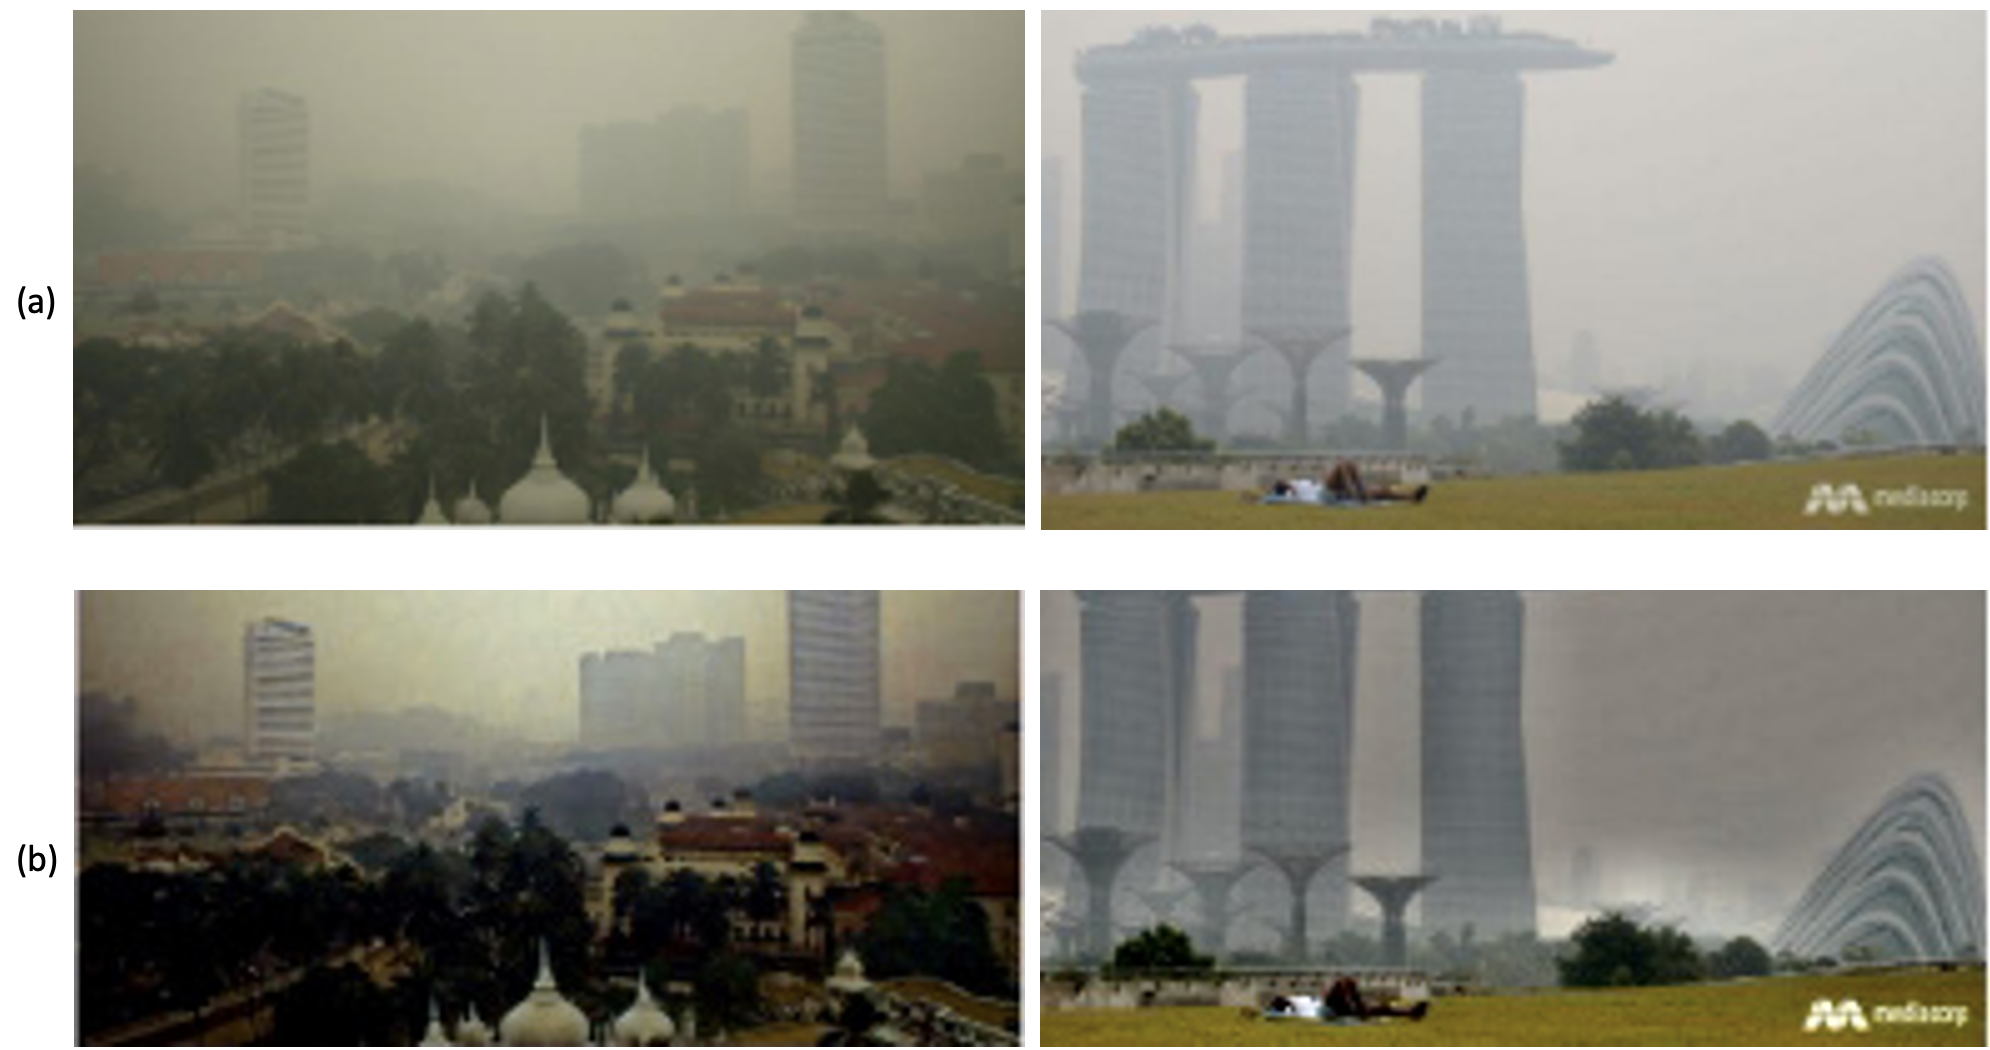
\includegraphics[width=1.0\linewidth]{f.png}
	\caption{Failure case of the proposed method. (a) Input Hazy image (b) Dehazed Image}
	\label{f}
\end{figure}

\section{Summary} \label{con}
The core contribution of this work is in twofold: (I) improve the estimation of transmission map and atmospheric light and (II) reduce computational complexity. The framework of the algorithm relies on DCP and Rayleigh scattering, which have solid mathematical foundations. The atmospheric light is estimated through a \textit{min, avg and max} analysis on the three colour channels while computation of the transmission map is calculated using Rayleigh scattering to form a scattering coefficient.  Finally, a qualitative and time complexity comparison show that the proposed method can effectively dehaze while achieving an excellent computational speed. However, there are still some limitations in our approach as shown in Figure~\ref{f}: (I) a small percentage of artifacts exits in the dehazed image, and (II) extensive optimization of the transmission map is needed. Thus, there is motivation for future research. \textbf{Published in \emph{IEEE ACCESS, JCR Q2 }}


\chapter{Multi-scale Haze Removal via Residual Network}
The scattering of climatic particles significantly alters images captured under unfavorable weather situations. Single image dehazing aiming to retrieve clear images from obscure images acquired under these conditions is an ill-posed problem. However, the advancement of technology has led to the publication of several dehazing algorithms with a significant focus on algorithms that estimate both the transmission map and the atmospheric light using the atmospheric scattering model\citing{a45}. Even though these algorithms achieve satisfactory results, they pose some limitations due to their hand-crafted features, e.g., dark channel, maximum contrast, and color disparity \citing{c1,c2,z1}. 
This chapter proposes a novel end-to-end algorithm to restore a hazy image using a residual-based deep CNN straightforwardly to address the drawbacks of traditional dehazing methods. The proposed algorithm is non-subject to the climatic dispersing model, yet it learns the mapping relationship within the hazy input image and their corresponding transmission map. The network architecture constitutes a convolution kernel and multi-scale fusion layers in extracting relevant features in predicting a holistic propagation map. Ultimately, we obtain the residual image and circumvent the loss of information using a residual network. We synthesize a dataset comprising hazy pictures and their identical transmission map from the NYU Depth dataset to train the network. Comprehensive empirical results demonstrate that the proposed technique outperforms multiple conventional algorithms. In summary, our contributions in this chapter are as follows:



\begin{itemize}
	\item This work presents a simple but effective end-to-end deep learning network to estimate the transmission map and atmospheric light directly without any dependency on the atmospheric scattering model.    
	\item  This work proposes a residual network to remove halos and speed up computation whiles maintaining texture features.  
	\item This work synthesizes indoor and outdoor datasets for our experiment to evaluate the method's efficiency. 
	
\end{itemize}
The remainder of the chapter is summarized as follows: The proposed approach and its implementation are addressed in Section\ref{3}. Section\ref{4} demonstrate empirical results and quantitative interpretation using performance metrics. Section\ref{5} concludes this study.

\begin{figure}[H]
\includegraphics[width=0.9\linewidth]{17.png}
\caption{Framework of the proposed image dehazing algorithm. The network principally consists of three modules: feature extraction, multi-scale mapping, residual learning, and fully connected layers
}
\label{fig:3}
\end{figure} 

 
\section{ Preliminaries}
In this section, we present concepts such as haze degradation model and CNN used for the framework of the proposed technique for single image dahazing.
\subsection{Haze Degradation Model}
The formation of haze images has been described by various research.The extensively used standards constitute an additive model and a haze degradation model. In this chapter, we utilize the latter to generate a trainable end-to-end deep neural network. The analytical formulation is written as follows: 
 \begin{equation}
I(x)= J(x)t(x) +A(1-t(x))
\end{equation}
where $x$ represents the position of a pixel in the image. The hazy image is denoted by $I$, $J$ is the haze free image to be recovered, $A$ is the global atmospheric light, $t$ represents the transmission map depicting the part of atmospheric light that enters the camera. The haze free image $J$ can be retrieved after $A$ and $t$ are adequately calculated. The analysis above shows that we must first estimate the transmission map and atmospheric light to obtain a haze free image. In this chapter, the haze formation model is employed to fabricate training pairs of hazy patches to evaluate our proposed method. This chapter builds a deep neural network to calculate the transmission map using the hazy input mage. That is, the algorithm takes a hazy input image and outputs its corresponding transmission map. In this chapter, the haze formation model is employed to fabricate training pairs of hazy patches to evaluate our proposed method. Finally, we recover a haze free image according to the estimated transmission map. 



\section{Network Design} \label{3}
In this section, we introduce the architecture of the proposed network. As discussed earlier, we build an end-to-end network that does not depend on the atmospheric scattering model to automatically study the mapping correlation between the dehazed image and the hazy input image. The algorithm is based on JinJiang\citing{a98} work with a few crucial distinctions such as:
\begin{itemize}
    \item Compared to their method, our approach adopts a linear translation variant filter to enhance further the propagation map.
    \item  The architectures are distinctive.
	\item Finally, we train our network by implementing the standard L2 loss with the perceptual loss function. 	
\end{itemize}
Figure~\ref{fig:3} highlights our network's architecture, which essentially consists of four progression modules: (I)feature extraction layer, (II) multi-scale context aggregation,(III) Residual network, and (IV) fully connected layers. In the following subsections, we introduce the proposed network architecture features, loss functions, and the training approach in details.
\begin{figure}[H]
\includegraphics[width=0.8\linewidth]{18.png}
\caption{(a) Rectified Linear Unit (ReLU) (B) Bilateral Rectified Linear Unit (BReLU)}
\label{fig:4}
\end{figure} 

\subsection{Estimation of Atmospheric Light and Transmission map}
As discussed in the literature work, traditional dehazing algorithms estimate the transmission map and the atmospheric light based on a strong assumption or a constant value. Despite visually compelling results, the dehazed image contains some artefacts. Estimating the transmission map from a hazy input image is deemed a pixel-level image regression assignment. In other words, the purpose is to learn a pixel-wise non-linear mapping from a provided input image to its corresponding transmission map by depreciating the loss among them. Our method adopts three sequential two-layer end-to-end convolution networks compared to the traditional transmission map estimation using the haze degradation model. The layers work as a two-set feature extraction unit to retrieve important information from the hazy input image.  This approach improves on the level of accuracy of the transmission map. 
\subsubsection{Feature Extraction}
Our algorithm's first phase has six layers responsible for extracting haze relevant features using a 2D convolutional kernel. In the convolution layer, a hazy patch of resolution 16x16 from the input layer is convolved with a kernel size of 3 to achieve a feature map of 16x14x14. The second layer segments the feature map's dimension from the preceding layer. Using Maxout\citing{a99}, the next layer generates a non-linear map while reducing the feature map's size and enhancing the network's performance by eliminating multicollinearity. This layer calculates the highest value of individual pixels from the sliced feature maps obtained in layer 2 to achieve a single feature as defined below: 
\begin{equation}
f_{ \alpha,j}(x)=\underset{i \epsilon {\big[j*k,k(j+1) \big]}}{Max} f( \alpha-1)_i (x), j \epsilon [1, \beta] 
\end{equation}	
where $j$ is the index of the feature map in the $ \alpha_{th}$ layer, $i$ denotes the index of the future map in the previous layer $(\alpha-1)_{th}$. The aggregate amount of feature maps is indicated by $\beta$ in the $ \alpha_{th}$ layer where $\beta = \alpha-1$. 
\par
To increase non-linearity in the output, an activation function which is the last component of convolution is applied. Most CNN-based image dehazing algorithms have recently applied RELU as the activation function to address the vanishing gradient puzzle. However, since image dehazing is an image restoration problem, RELU is less suitable because RELU was designed for classification problems. This work selects a Bilateral Rectified Linear Unit (BReLU)\citing{a50} as the convolution layer's activation function. Figure~\ref{fig:4} exhibits the distinction between the two activation functions. The final convolution is obtained as:
\begin{equation}
	F_n= min(t_{max}, max(t_{min,}w_n*F_{n-1}*B_n)),
\end{equation}	
where $B$ represents the offset value, $n$ represent the feature map of the last layer. $t_{min}$ and $t_{max}$ are the marginal value of the activation function(BReLU) (note that $t_{max=0}$ and $t_{max=1}$ in this dissertation). 


\subsubsection{Multi-Scale Multi-feature fusion }
When perceiving an image, we usually enlarge it to identify its regional and global components. This method proves that distinct layers are essential for deducing the corresponding haze depth from a single image when supplementary data is needing. Two strategies are adopted to obtain features in a large receptive field: (I) intensifying the network and (II) increasing the dimension of convolutional kernels. Theoretically, features obtained from high-level layers of a network have a more extensive receptive field on the input image. Expanding the kernel dimension can also receive further comprehensive information. However, this strategy creates exponential growth of learnable parameters. Dilated convolution presents a unique procedure to achieve multi-scale context by utilizing different rates to address this problem. This method expands the receptive field without extra parameters to efficiently learn more extensive, powerful, and abstract information. Also, dilated convolution is intelligent in clustering multi-scale contextual learning without dissipating resolution or interpreting resized images. Achieving a concrete haze estimation is not merely attainable. The characteristic from upper-level layers is anticipated to drop ineffective features, such as haze. More extensive networks also suffer a degeneration difficulty: an expansion in the network depth results in efficiency saturation. This issue is not induced by overfitting. Figure~\ref{dil} demonstrates two-dilated convolution using a kernel size 3×3 at a dilation rate of two. Consequently, every component in the feature map after dilated convolution has a receptive field of 7×7. Overall, the size of the sensory range of 3×3 filters with different dilation rate can be computed as follows:
\begin{equation}
	R_f=(2^{i+2} -1) * (2^{i+2} -1), i= max {j|2^j \leq f, j \epsilon N}
\end{equation}	
where $N$ describes the collection of real numbers. The padding rate is set as $R_f/2$ in the corresponding region to make the obtained feature map's dimension consistent. 
\begin{figure}[H]
\begin{center}
\includegraphics[width=1.0\linewidth]{dil.png}
\caption{An illustration of dilated convolution. The input feature map is of size 9×9 and padded with 3 pixels. The padding value is zero. The convolution kernel is of size 3×3, and its dilation rate equals 2. Each element in the resulting feature map has a receptive field of 7×7 [64]}
\label{dil}
\end{center}
\end{figure} 
The efficiency of adopting multi-scale mapping to extract low and high-level haze-relevant features has improved the extraction of information in a more significant receptive field. This method expands the receptive field without any additional elements to learn both low and high features. Inspired by its excellent implementation, in this chapter, we adopt parallel sub-layers with the receptive field of 3×3, 5×5, and 7×7 in the fourth layer to extract both faint and high-level data from the feature map resolution 14×14×4. The fifth layer performs the highest value selection of individual patches of the feature map from layer 4 using a 2x2 non-overlapping window to obtain 8×8×48. The last layer converts the input information from layer 5  to get a final feature map with dimensions 1x1. The output data has a size limited to [0,1]. The propagation map is learned from the output data. 
\begin{figure}[H]
\begin{center}
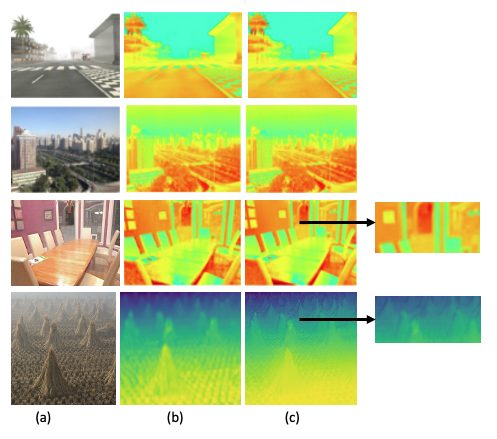
\includegraphics[width=0.9\linewidth]{19.png}
\caption{Comparison of $t$ before and after refinement (a) Hazy Image  (b) Transmission map $t$ (c) Refined Transmission map}
\label{fig:5}
\end{center}
\end{figure} 
\subsection{Transmission map refinement} 
In this part, we additionally intensify the correctness of the propagation map, using a guided filter. This measure reduces synthetic textures and blocking artefacts created in the ultimate image, as shown in Figure~\ref{fig:5}. The refinement filter is constructed on an immediate translation variant where the filter takes an input image $I$, guidance image $P$ and outputs $X$. We represent a linear translation variant filter as follows:

\begin{equation}
t_{(x1)}=\sum_j w_{i,j} \cdot (P)\cdot I_j
\end{equation}
where $w_{(i,j)}$ is a filter mask kernel with a pixel ratio $i,j$, $I$ is the input image and $P$ is the guidance image. To depreciate the error included in remodelling $I$ and $P$, we introduce mean and variance.  
\begin{equation}
x_i=a_k P_i+b_k\ \forall i\epsilon w_k
\end{equation}
where:
\begin{equation}
a_k= \frac{\frac{1}{|w|} \sum i  \epsilon w_k P_i I_i -\mu_k \bar I_k}\, {\sigma_k^2  + \epsilon}
\end{equation}
\begin{equation}
b_k=  \bar I_k - a_k \sigma_k^2 \mu_k
\end{equation}
$\bar{I}_k $ is the mean of the input image $I$ in window $w_k$. $\epsilon$ is the regularization parameter. Figure 5 exhibits the difference within the transmission map and the refined transmission map utilizing the refinement filter.
\begin{figure}[H]
\begin{center}
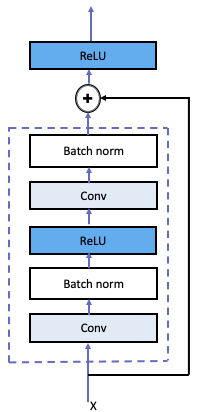
\includegraphics[width=4.6 cm]{20.png}
\caption{Residual network element for the proposed method. The first convolutional layer outputs its learned features x, which are sent to the second and third convolutional layer for learning residual features $F_{(x)}$. $F_{(x)}$ and $x$ are then fused using a sum operation to form the target features $H_{(x)}$}
\label{fig:6}
\end{center}
\end{figure} 
\subsection{Residual Block }
Achieving a concrete haze estimation is not merely attainable. The characteristic from upper-level layers is anticipated to drop ineffective features, such as haze. A network's depth is highly imperative, but deeper networks present degradation problems: an expansion in the network depth results in efficiency saturation. This degradation problem does not result from over-fitting. In image restoration, feature maps acquired at high-level layers always lose small data. Rather than predicting that every layer will instantly fit a wanted underlying mapping, we straightforward allow some layers to include a residual mapping. 
In this chapter, we design a residual block proposed by RESNET\citing{a100} to learn the residual functions from the preceding layers effectively. We employ the RELU function to activate the input and output components from different convolution to obtain the final output layer. As presented in Figure~\ref{fig:6}, the structural block in ResNet, which is the foundation of our design, is described as follows:
\begin{equation}
	u=F(x,W_i)+x,
\end{equation}
where $F(x, W_i)$ is the residual network to be learned. $x$ and $u$ are input and output characteristics of a distinct layer. The block of our proposed residual network consists of 2 convolution layers and 8 BN+Conv layers. The first layer outputs determine feature $x$, which goes through the middle layers (BN+Conv layers) for learning residual features $F(x)$. In this dissertation, we employ an input image with size 16x16 and kernel filter size of 3x3. We obtain the output feature with a ReLU activation function. Finally, we use 3×3×16 filters size to rebuild the feature map to get the residual image.
\begin{figure}[H]
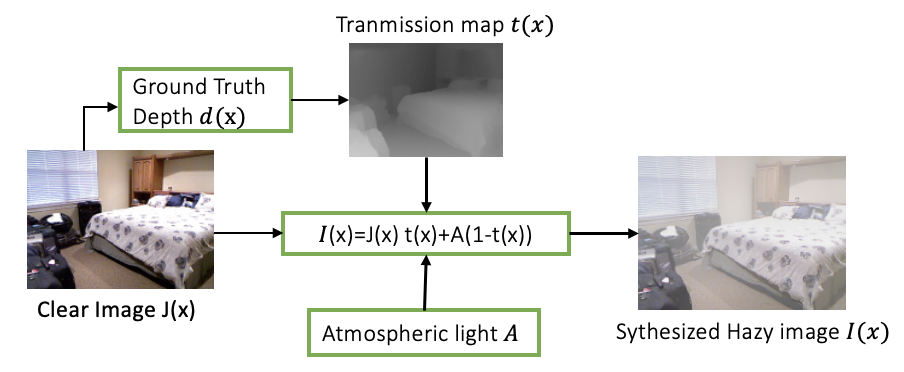
\includegraphics[width=1.0\linewidth]{22.png}
\caption{Training dataset generation Framework}
\label{fig:8}
\end{figure}
\subsection{Fully Connected Layers}
At the end of the proposed network,  we employ fully connected  (FC)  layers to obtain the transmission map using features from stacked convolutional layers.  The feature maps of the last convolutional layer are flattened and supplied into the FC layers. To improve over-fitting, we adopt a dropout regularization method that randomly places a part of the hidden neurons to zero during training.  The abandoned neurons do not provide the forward propagation and are not accepted in the back-propagation method. Conclusively, the FC layers present a single value describing the haze transmission at the intermediate pixel of individual input of hazy patches.   

\subsubsection{Loss function }
We minimize the mapping relationship between the RGB value and its respective transmission medium through supervised learning to estimate the transmission map. Earlier works have recorded that it is compelling to select the suitable loss function when training reconstruction network. Algorithms that use L2 error creates a distorted output. Modern results have confirmed that high-quality images are obtained by employing perceptual loss functions based not on contrasts between pixels but preferably on distinctions between significant level image feature representations derived from pre-trained CNN. Motivated by\citing{a101}, we decrease the weights of the proposed network  by combining perceptual loss of $L_P$ and $L_E$ reconstruction error as follow:
\begin{equation}
	L=L_E +\lambda_pL_p,
\end{equation}
where $L_E$ is represents the standard L2 loss function defined as :
\begin{equation}
	L_E= \frac{1}{CWH}\sum_{c=1}^C \sum_{w=1}^W\sum_{h=1}^H \big\| G(I(c,w,h),\Theta ) -I_t(c,w,h) \big\|_2
\end{equation}
Here, $w, x, h$ is the resolution of the input hazy image $I$ in C-channel. $I_{(t)}$ is the scene radiance to be obtained. $\theta$ is represents the network parameter, and $G$ is the network function. $L_{(p)}$ works by finding the mean of the total squared errors of pixels. The principal purpose is to lessen the perceptual disparity between the reconstructed image and the ground truth. In this dissertation, $L_{(p)}$ is grounded on VGG-16 architecture:
\begin{equation}
	L_E= \frac{1}{C_v W_v H_v}\sum_{c=1}^{C_v}\sum_{w=1}^{W_v}\sum_{h=1}^{H_v} \big\| \phi_V(G(I,\Theta )) -\phi_V(I_t) \big\|_2
\end{equation}
where $\phi_V$ is activation map of shape ${C_v}{W_v}{H_v} $. 
\begin{figure}[H]
\begin{center}
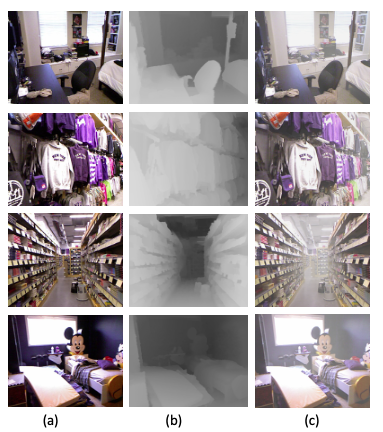
\includegraphics[width=0.8\linewidth]{21.png}
\caption{Examples of synthetic hazy images generated. (a) Clear images used as ground-truths (b) Transmission maps used to estimate the depth scene  (c) Hazy images  obtained using hazy image model.}
\label{fig:7}
\end{center}
\end{figure}
\section{Experimental Results}\label{4}
 In this section, we verify the effectiveness of our proposed algorithm on two artificial datasets. We conduct a qualitative examination of the proposed method with different state-of-the-art algorithms on an indoor and outdoor synthetic dataset using three other blind evaluation metrics. 
\subsection{Synthetic Dataset( Training and Test Dataset)}
An excellent network depends on various parts: (I) exceptional architecture, (II) comprehensive implementation, and (III) training process.  Numerous image restoration and enhancement assignments benefit from the constant efforts for standardized benchmarks to compare unique proposed algorithms under the exact requirements. It is commonly unachievable to obtain the equivalent visual scene with and without haze,  while all other environmental circumstances stay the same.  Therefore, modern dehazing algorithms generally create their training sets by generating hazy synthetic images from hazy free images: they first obtain depth maps of the clean images by either utilizing available depth maps for depth image datasets or estimating the depth and then create the hazy images by computing  (1) haze removal models could then be trained to revert haze free images from hazy ones.
A substantial number of training units consisting of hazy patches and their identical haze transmissions are needed. However, a significant shortcoming in using the CNN reconstruction network for image dehazing is the scarcity of hazy datasets. Based on the physical model and the assumption that the transmission map of an image is constant and it is autonomous of the transmission map in a small patch, we generate a synthesized training dataset with their identical transmission map as shown in Figure~\ref{fig:8} as follow:

\begin{equation}
	I^p_{(x)}=H^p_{(x)}t+A(1-t)
\end{equation}
where $t$ is an arbitrary transmission map, $A$ is the atmospheric light and is the haze free patch. To subdue imbalance in the synthesis we set the atmospheric light $A=[k,k,k]$ where $K\epsilon[0.8,1.0]$.
 This work randomly samples 12,00 indoor images and their corresponding depth maps and select 50 patches with a dimension of 16x16 from the individual image in the NYU dataset. Thus, 60,000 simulated hazy patches are collected. Figure~\ref{fig:7} displays some samples of synthesized hazy images generated from the NYU dataset. The dataset consists of multiple indoor scenes photographed by RGB and depth cameras from Microsoft Kinect. It comprises 1449 densely labelled pairs of aligned RGB and depth images, 464 different scenes taken from 3 cities and 407,024 new labelled frames. We adopt an Indoor Training Set (ITS), and Synthetic Objective Testing set (SOTS) from RESIDE\citing{a102} in our experiment to train the network. 
\begin{figure}[H]
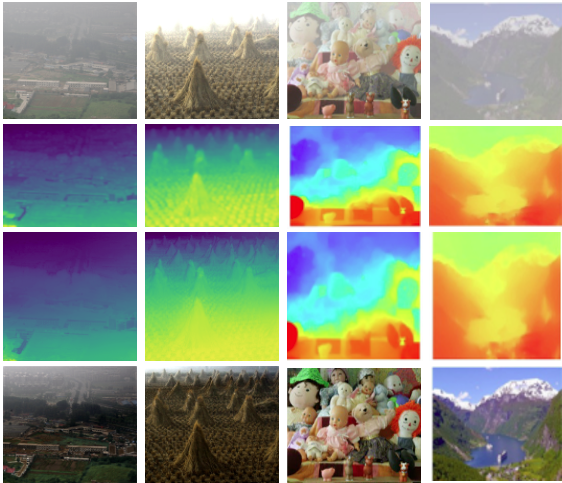
\includegraphics[width=0.9\linewidth]{23.png}
\caption{Sample dehazing results using the proposed method. Row 1. Input hazy images. Row 2. Estimated transmission map. Row 3. Refined transmission map Row 4. Dehazed Image}
\label{fig:8}
\end{figure}
\subsection{Training Detail}
To subdue over-fitting, decrease noise volume, and make the training process robust during training, we attach a Gaussian Noise layer to the input layer. Weights are initialized to a Gaussian distribution with a mean of 0.0 and a standard deviation of 0.001, taken arbitrarily. We use the Adam optimization method with $\beta_1=0.99, \beta_2=0.999$ to train our network for 300,000 iterations. We set the learning rate to $2*10^{-4}$, batch size to 1, and the epoch to 10. The proposed algorithm is implemented in TensorFlow on a computer with a NvidiaTitan-X GPU.


\subsection{Quantitative Evaluation}
We evaluate our algorithm's dehazing performance on a synthetic dataset and compare the proposed method with state-of-the-art methods, including DCP\citing{a33}, AOD$-$Network\citing{a58}, Jin's method\citing{a98}, Zhu's method\citing{a34}, FFA-Net\citing{a54}, Cai's method\citing{ a50}, NBPC\citing{80}, MSCNN\citing{nw1}. We measure the performance using  Peak Signal-to-Noise Ratio (PSNR) and Structural Similarity (SSIM) and Fog Aware Density Evaluator (FADE) as shown in Table~\ref{Tab6} and ~\ref{Tab7}. For the avoidance of any inclinations, we use an equivalent dataset to retrain the data-driven method. Due to the absence of ground truth in real world images, we assess real-world images qualitatively. Fog Aware Density Evaluator (FADE) is a reference evaluation method that predicts a hazy scene's visibility from a single input image without the respective haze free image. This method only makes quantifiable deviations from statistical regularities observed in natural hazy and hazy free images. A low FADE value indicates a high potency of the algorithm to eliminate haze. PSNR is a full reference evaluation method, which uses three parameters:(I) the new apparent edge ratio (II) normalizes gradient of the visible edge and the (III) proportion of saturated white or black pixels. This method demands clear images, and the photos to be evaluated. We define PSNR as:
\begin{equation}
	PSNR = 10log_{10} \frac{ 255  }{\sqrt\big| X_{in}-X_{out}\big|^2}
\end{equation}

where $X(in)$ and $X(out)$ represent the hazy output and the hazy image model respectively. A dehazed image with a high contrast depicts a unique algorithm. 
SSIM evaluation method, measures the similarities between the clean image and the image in three ways: (I) brightness, (II) contrast, and (III) structure. The definition of SSIM is as follows:

\begin{equation}
	SSIM= \frac{(2\mu_{ x_{in}}\mu _{x_{out}}+ \theta _2) (2 \sigma _{x_{in} x_{out}}+ \theta _2)}  { ( \mu ^2_{ x_{in}}+ \mu^2_{x_{out}}+ \theta_1)( \sigma^2_{x_{in}} +\sigma^2_{x_{out}} +\theta_1)      }
\end{equation}

where $\theta_1$ and $\theta_2$ are constant values utilized in the avoidance framework vulnerability created by a denominator of 0 with a  value range of [0,1]. A large value represents higher similarities between the ground truth and dehazed image. $\mu_{ x_{in}}$ and $ \mu_{ x_{out}}$ are the average of the hazy image output $ x_{in} $ and the hazy image model $x_{out}$ respectively. $\mu^2_{x_{in}}$ is the variance  of $ x_{in} $ . $ \mu^2_{x_{out}}$ is the variance of the hazy image model $x_{out}$. Table 1 and 2 represents the average values for the evaluation metric used in our quantitative analysis. It is evident from experimental outcomes that our proposed technique achieves the best score in FADE, PSNR ,and SSIM for outdoor and indoor images.

\subsubsection{Indoor dataset Analysis}
In this section, we examine our algorithm with the fore discussed conventional dehazing algorithms using indoor images. Figure~\ref{fig:8} 10(a) - 10(g) shows the proposed algorithm's dehazing results with that of 5 state-of-the-art restoration methods, namely: DCP\citing{a33}, AOD$-$Network\citing{a58}, Jin's method\citing{a98}, Zhu's method\citing{a34}, FFA-Net\citing{a54}. DCP\citing{a33} approach exhibits outstanding results on removing in-homogeneous haze. However, the highest illuminated regions in the images appear over-saturated. The image also bears some artefacts. In AOD$-$Network\citing{a58}, images do have some level of quality, visual effects. However, the results prove the images have some haze, as shown in Figure~\ref{fig:8}(C1, C2, C3). In Zhu's method\citing{a34}, images obtained are over enhanced; hence, the dehazed image's hues appear distorted. 
\begin{figure}[!htb]
	\centering
	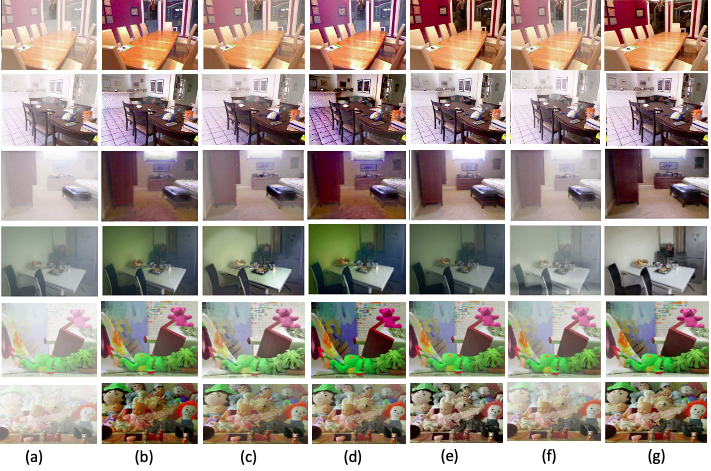
\includegraphics[width=1.0\linewidth]{24.png}
	\caption{Comparison of the proposed method with traditional algorithms using Indoor synthetic images. (a) Input hazy image;(b) DCP [56] ; (c) AOD−Network [81]; (d) Jin method [171]; (e) Zhu method [57]; (f) FFA-Net [77]; (g) Proposed method.}
	\label{fig:9}
\end{figure}

For example, in Figure~\ref{fig:8}(d3), the wall's colour is over-saturated; consequently, it appears yellowish instead of whitish. In FFA-Net\citing{a54}, images appear to have some haze residues. In contrast, the proposed algorithm generates high-quality essential outcomes with fewer artefacts. 
\begin{figure*}[!htb]
	\centering
	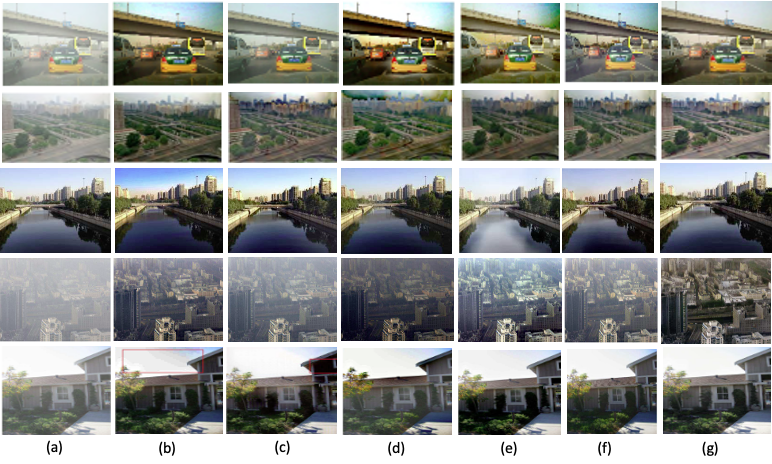
\includegraphics[width=1.0\linewidth]{25.png}
	\caption{ Comparison of the proposed method with traditional algorithms using Outdoor synthetic images. (a) Input hazy image;(b) DCP [56]; (c) AOD−Network [81]; (d) Jin method [171]; (e) Zhu method [57]; (f) FFA-Net [77]; (g) Proposed method.}
	\label{fig:10}
\end{figure*}


\subsubsection{Outdoor dataset Analysis}
Figure~\ref{fig:10}(a) - (g) shows the after-effects of the proposed method in comparison with that of DCP\citing{a33}, AOD$-$Network\citing{a58}, Jin's method\citing{a98}, Zhu's method\citing{a34}, FFA-Net\citing{a54}. In the results of DCP\citing{a33}, Figure~\ref{fig:10}(b), the sky areas are over-saturated, and the images bear some artefacts. AOD$-$Network\citing{a58} produce excellent results with the best visual effects. However, the sky regions appear to have small halos. Jin's method\citing{a98} is the most advanced network; therefore, its results are excellent. Its major drawback is the shift in colour in heavily dense areas. Zhu's method\citing{a34} algorithm produces excellent results, but low light images produce darker results. The performance of FFA-Net\citing{a54} algorithm is deficient. Images dehazed using the algorithm still has some amount of haze. The FADE value is very high compared to the original image. Empirical results indicate that all algorithms somewhat show a noticeable enhancement in the hazy region but  Overall, our method achieves the highest satisfactory results. We attribute the significant differences to the amount of haze residue and various climatic situations

\begin{table}
	\centering
	\caption{The objective image quality comparison of dehazing results of Indoor image - Figure~\ref{fig:9} The value in the table are averages of all images}
    \begin{tabular}{|p{49pt}|p{50pt}|p{50pt}|p{52pt}|p{52pt}|p{52pt}|p{52pt}|p{52pt}|}
    
	\hline\textbf{Parameters}	& \textbf{DCP[56]}& \textbf{AOD[81]} &  \textbf{Jin method[171]}	& \textbf{Zhu method[57]} & \textbf{FFA-Net[77]}  &  \textbf{Proposed Method}\\
	\hline
	$ PSNR$&28.701&28.148&27.492&28.001&29.232&30.121\\
		\hline	
	$SSIM$&0.979&0.958&0.912&0.911&0.963&0.985\\
		\hline	
	$FADE$&0.568&0.811&0.732&0.545&0.792&0.534\\
	\hline	
\end{tabular}
	\label{Tab6}
\end{table}

\subsubsection{Real-world hazy images Analysis}
Figure~\ref{fig:11}(a) - (g) and Figure~\ref{fig:cnn1}(a) - (g) shows the results and comparisons on real world hazy images obtained from the Internet. Admittedly from an initial glimpse, all algorithms produce excellent results. However, some dehazed images are over saturated and contain haze residues. In the results of DCP\citing{a33} Figure~\ref{fig:11}(b1)- (b4) and AOD$-$Network\citing{a58} Figure~\ref{fig:11}(c1)- (c4), the dehazed images contain some amount of haze residue in dark regions. In Jin's method\citing{a98} Figure~\ref{fig:11}(d1)- (d4), images appear over-saturated; therefore, they contain halo artefacts, and the sky regions are dark. In Zhu's method\citing{a34} Figure~\ref{fig:11}(e1) - (e4), the dehazed image is not clear as a result of colour variation and the volume of haze. In FFA-Net\citing{a54} algorithm, the dehazed image has some remaining haze, as shown in Figure~\ref{fig:11}(f1)- (f4). Overall, our proposed method generated promising results with fewer colour distortions.

\begin{figure*}
	\centering
	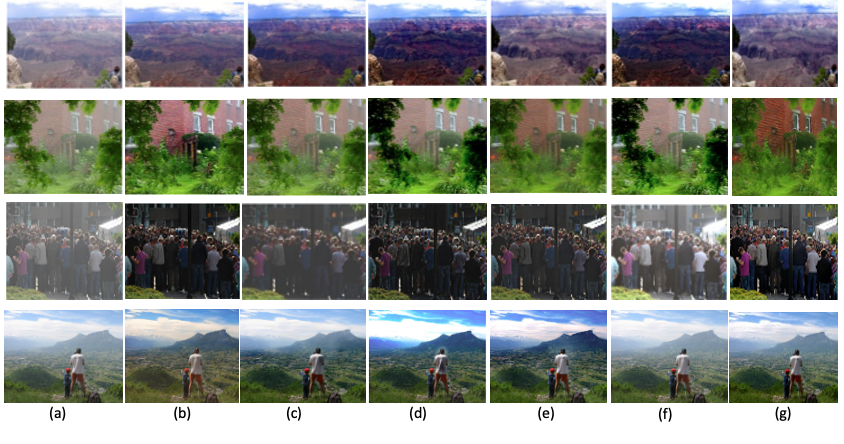
\includegraphics[width=0.9\linewidth]{26.png}
	\caption{ Visual comparison of results on real world hazy images: (a) Input hazy image;(b) DCP [56]; (c) AOD−Network [81]; (d) Jin method [171]; (e) Zhu method [57]; (f) FFA-Net [77] ; (g) Proposed method.}
	\label{fig:11}
\end{figure*}

\begin{table}
	\centering
	\caption{The objective image quality comparison of dehazing results of Outdoor image - Figure~\ref{fig:10} The value in the table are averages of all images}
    \begin{tabular}{|p{49pt}|p{52pt}|p{52pt}|p{52pt}|p{52pt}|p{52pt}|p{52pt}|p{52pt}|}
    
	\hline\textbf{Parameters}	& \textbf{DCP[56]}& \textbf{AOD[81]} &  \textbf{Jin method[171]}& \textbf{Zhu method[57]} & \textbf{FFA-Net[77]}  &  \textbf{Proposed Method}\\
	\hline
	$PSNR$&  28.423 & 28.013 & 27.932 & 27.841 & 30.015 & 31.051\\
		\hline	
	$SSIM$& 0.936 & 0.973 & 0.952 & 0.924 & 0.942&0.989\\
		\hline	
	$FADE$& 0.562 & 0.743 & 0.899 & 0.733 & 0.498&0.478\\
	\hline	
\end{tabular}
	\label{Tab7}
\end{table}
\begin{figure*}[!htb]
	\centering
	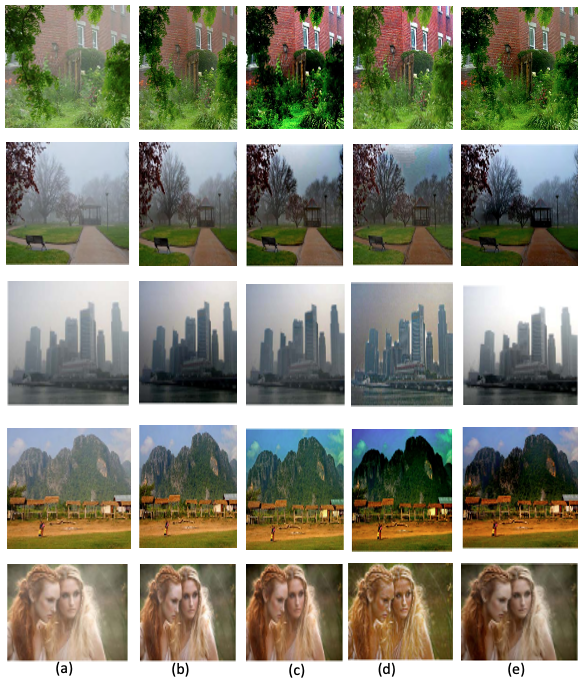
\includegraphics[width=0.9\linewidth]{nw1.png}
	\caption{ Visual comparison of results on real world hazy images: (a) Input hazy image;(b) DehazeNet[75]; (c) MSCNN [70]; (d) NBPS [71]; (e) Proposed method.}
	\label{fig:cnn1}
\end{figure*}
\subsection{ Limitation}
Our proposed method trains on a  set of the synthetic dataset generated using the haze physical model equation. Because the hazy physical model does not account for night time hazy images, the proposed method is less effective in removing nighttime images with haze. Furthermore, due to the heterogeneous nature of extracting characteristics and estimating the transmission map using an end-to-end network, the computational time is high.

\section{Summary}\label{5}
In this dissertation, we present a residual-based network for single image dehazing. This work's core contribution is to advance the transmission map estimation and atmospheric light using an end-to-end network. The overall architecture comprises four sequential modules: (I) feature extraction layer, which uses 2D convolution kernels to obtain information from the input image. (II) multi-scale context aggregation, which adopts enlarged convolution to retrieve valuable highlights in various receptive fields without dissipating resolution, (III) residual network reduces the loss of extracted data while increasing the network vital level features. (IV) fully connected layers. Our algorithm's framework does not depend on the physical model. However, it efficiently eliminates haze from an input image as opposed to traditional dehazing algorithms. The network learns by minimizing the mapping relationship between the RGB value and its respective transmission medium. Finally, to assess our method robustness, we generate outdoor and indoor synthetic hazy images using NYU2 dataset. We generate datasets to train the proposed network from clear photos and their respective transmission map by simulating the physical model. Comparing experimental results with traditional dehazing algorithms reveals that the proposed method can effectively produce a significant enhancement in hazy regions. \textbf{Published in the Proceedings of the 3rd International Conference on Image, Video and Signal Processing}


\chapter{Single Image Dehazing with Lab Analysis}
In summary, this chapter proposes a real time effective dehazing algorithm for hazy surveillance images. This algorithm is based on histogram equalization and a filtering manipulation on the Lab color channel. In the proposed algorithm, the input RGB image is transformed into Lab color channel then, contrast limited adaptive histogram equalization (CLAHE), and a smoothing operation is applied respectively and simultaneously on the luminosity layer and the two color channels (a and b) of the Lab color space. The channels are merged back to obtain a new enhanced image
\section{Introduction}
Images captured in the opened environment usually experience low complexities and distorted colors due to turbid medium (e.g., dust, smoke, haze, fog) in the atmosphere. In these circumstances, perceivability distance is diminished due to the absorption and dispersing of light by the atmospheric particles. The light reflected from the object in the caught scene is attenuated by scattering along the line of sight of the camera. Image dehazing has two main principal goals: (1) enhancing the scene's perceivability and amending the loss of light force caused by apparent aerosols. (2) Improving photography and computer vision application. In medical image processing, coding, and machine vision, image enhancement is essential for human visual observation.
However, dehazing is a challenging problem for image processing and the computer vision domain because of its dependence on the unknown scene depth. In recent years conventional research work has concentrated on the most proficient method to create quality dehazed images.  These algorithms can be classified into two groups\citing{60,70,80}: (1) Non model based enhancement techniques (2) model based. Image enhancement under Non model based is done by using histogram equalization or adaptive histogram. Unfortunately, these methods do not maintain color fidelity and are not suitable for real time computer vision. Model based contrast enhancement techniques are based on the known depth and unknown depth. Histogram equalization applies stochastic probability distribution on individual channel level of color images. Consequently, histogram equalization has widely been adopted to enhance an image contrast or maintain image luminosity\citing{a103,a104}. It usually contains two primary steps: (I)smoothing and (II)stretching phase. Subsequently, the contrast is enhanced. The histogram equalization is broadly employed because of its uniformity. Images acquired by the visual framework are genuinely corrupted under cloudy and foggy climate, affecting detection, tracking, and image recognition\citing{l1,l2,l3,l4}. Thus, restoring the actual scene from a hazy image is of great significance.  
Overall, the image's high-frequency elements are combined with the image region whose contrast dramatically increases, such as its edge. The low frequency segments illustrate the low area of an image, including the sky region. The airlight element of the haze degradation model can be seen as the principal part of low frequency. The edge data of a hazy image is typically diminished due to the impact of haze. That is, the high frequency elements are minimized while the low frequency elements are enhanced. Therefore, improving the high frequency segments and minimizing the low-frequency segments of an image can enhance a hazy image.
To address this problem, we propose a real time effective dehazing algorithm for hazy surveillance images. This algorithm is based on Histogram and a filtering manipulation on the Lab color channel. In the proposed algorithm, the input RGB image is transformed into Lab color channel then, contrast limited adaptive histogram equalization (CLAHE), and a smoothing operation is applied respectively and simultaneously on the luminosity layer "L" and the two color channels (a and b) of the Lab color space. The channels are merged back to obtain a new enhanced image, which is then transformed back to RGB image. Experimental results show the effectiveness and the short computational time of the proposed algorithm.
\begin{figure*}
	\centering
	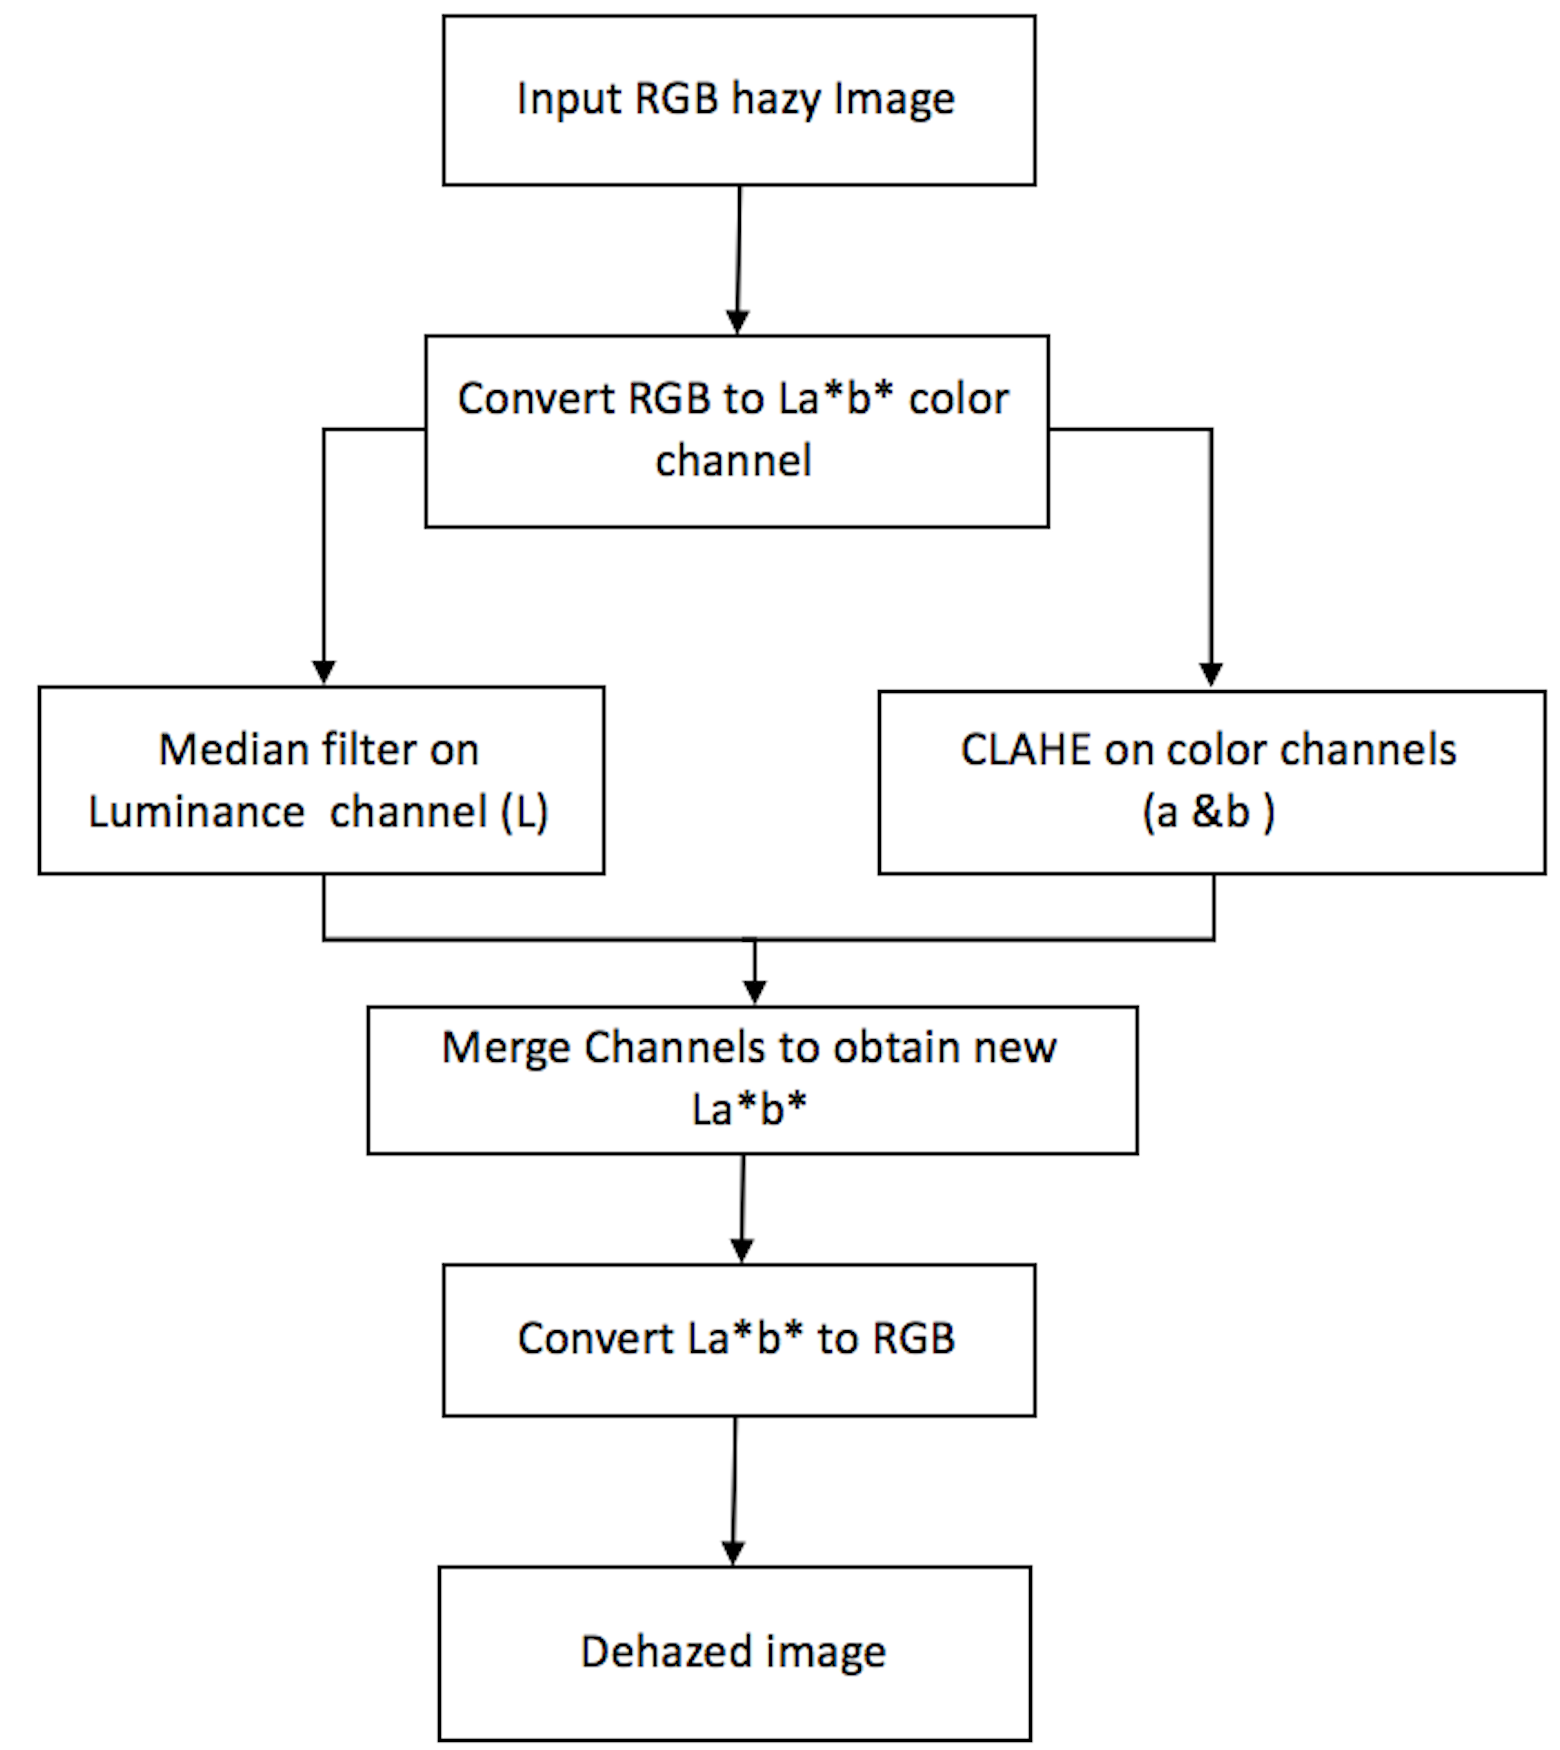
\includegraphics[width=0.6\linewidth]{27.png}
	\caption{Block diagram of proposed method.}
	\label{fig:12}
\end{figure*}

\section{Proposed Method}
Image contrast enhancement algorithms aim to increase the image's contrast and are widely adopted in image defogging, underwater image enhancement, and medical image enhancement. The foggy image histogram usually is circulated halfway since most pixels have large color values or gray values. Thus, the hazy image has low contrast and dynamic range. Intensity transforms a simple and effective method that enhances the appearance by redistributing the histogram. The histogram equalization algorithm improves the image by redistributing the histogram of the image to enlarge its dynamic scope. In contrast enhancement, local histogram equalization (LHE) and global histogram equalization (GHE) are adopted \citing{a105,a107}. Immediately applying HE algorithm on each color channel will alter the color composition of hazy images, resulting in the HE algorithm undergoing a color deformity problem.
Even though we can exclusively use the HE calculation to the depth channel to decrease the color deformity, the improved image also finds the difficulty of color degradation due to the intensity's control on all channels of the hazy image. However, for some hazy images with dense fog, the distinctness of the enhanced image acquired by the HE based algorithm is more substantial than different techniques.Several images acquiring methods use RGB color space as the criterion due to its brightness information. Consequently, the linear use of these elements usually cannot get the aspired outcome. Lab color space has a broad color range, and it can express all colors observed by human eyes and make up for the color saturation difficulty of RGB color space. 
This chapter proposes a real time single image dehazing algorithm based on Histogram and a filtering manipulation on Lab color channel. The proposed algorithm depends on three principal steps: (I) Converting RGB hazy image to Lab color channel (II) Enhancing the color channels (III) Converting enhanced lab image to RGB.  The proposed algorithm is efficient for real time single image dehazing. Experimental results show the effectiveness and the short computational time of the proposed algorithm. Figure ~\ref{fig:12} shows the flowchart of the proposed algorithm. 
\begin{figure*}
	\centering
	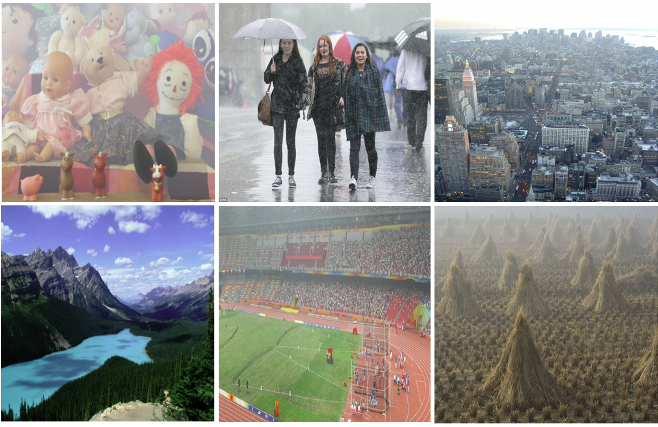
\includegraphics[width=1.0\linewidth]{28.png}
	\caption{Sample hazy images of our work.}
	\label{fig:13}
\end{figure*}
\subsection{Converting RGB to Lab}
The RGB color space is an additive color model where three color (R (red), G (green), and B (blue)) lights are complemented collectively in a single space to reproduce a wide array of potentially visible colors. The primary purpose of the usage of RGB color space is to present images in a computerized way. However, sometimes it is more satisfying to utilize different color spaces. In this dissertation, we adopt the Lab color channel for contrast enhancement of a hazy input image. 
The CIE defines the Lab color channel based on one channel for Luminance (lightness) and two color channels (a and b). Figure~\ref{fig:14} shows a block diagram of the Lab diagram. The $a$ layer indicates where the color falls along the red green axis, and the b layer indicates where the color falls along the blue yellow axis. $a$ negative values indicate green while positive values indicate magenta, and $b$ negative values indicate blue and positive values indicate yellow. The $L$ channel represents the darkest pixel at $L = 0$, and the brightest white at $L = 1$. The shading channels, $a$ and $b$, represents the genuine impartial dim values at $a = 0$ and $b = 0$. This color space is more qualified to numerous computerized picture controls than the RGB space, normally utilized as picture altering programs. For instance, the Lab space helps hone pictures and the evacuating relics in JPEG pictures or pictures from advanced cameras and scanners. In converting an RGB image to Lab color space image, we need XYZ color. The following equation gives the Lab color component\citing{a108}.

\subsubsection{STEP 1: Convert from RGB to XYZ}
The first step in the calculation of RGB from CIE XYZ is a linear transformation, which is carried out by a matrix multiplication[13].\\
\begin{equation}
\left[\begin{array}{ccc}
X \\
Y \\
Z\end{array} \right] = \left[ \begin{array}{ccc}
0.414253 & 0.357580 & 0.180423 \\
0.212671 & 0.715160 & 0.072169 \\
0.019334 & 0.119193 & 0.950227 \end{array} \right] \left[ \begin{array}{ccc}
R \\
G \\
B \end{array} \right] \\
\end{equation}
\subsubsection{STEP 2: Convert XYZ to lab}
Next we convert X, Y, Z  into lab color channel which is perceived in the three dimensions (L) for lightness and (a and b) for the color opponents green red and blue yellow. Luminosity layer L represents the darkest black at L = 0, and the brightest white at L = 100. Color channel a and b represents gray values at a=0 and b=0
\[\]

\begin{equation} L=116\bigg[h\bigg(\frac{Y}{Y_w}\bigg)-16\bigg] \end{equation} 

\begin{equation}a=500 \bigg[h\bigg(\frac{X}{X_w}\bigg)- h\bigg(\frac{Y}{Y_w}\biggl)\biggl]\end{equation}

\begin{equation}b=200 \bigg[h\bigg(\frac{Y}{Y_w}\bigg)- h\bigg(\frac{Z}{Z_w}\bigg)\bigg]\end{equation} 
\begin{equation}\text{where h(q)}=
\begin{cases}
\sqrt[3]{q} &\text{q} > 0.008856\\
7.787q+16/16 &\text{q}  \leqslant 0.008856
\end{cases}
\end{equation}

\begin{figure*}
	\centering
	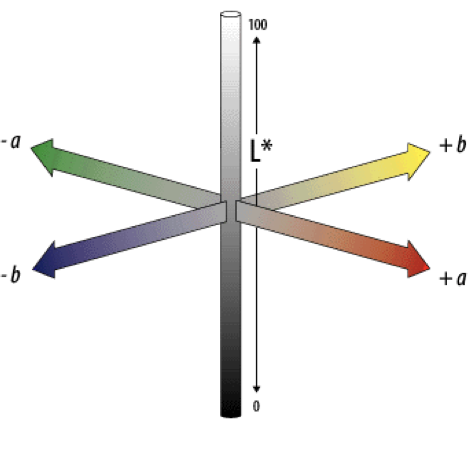
\includegraphics[width=0.7\linewidth]{29.png}
	\caption{Block diagram of lab color channel.}
	\label{fig:14}
\end{figure*}

\subsection{Enhancing the Color Channels}
In our proposed method, we enhance the two color channel (a and b) using Contrast Limited Adaptive Histogram Equalization (CLAHE). In contrast, with limited histogram equalization (CLAHE), the histogram is cut at some threshold, and then equalization is applied. Contrast limited adaptive histogram equalization (CLAHE) is an adaptive contrast histogram equalization strategy where the difference of an image is upgraded by applying CLAHE on little information locales called tiles instead of the whole image. The subsequent neighboring tiles are then sewed back flawlessly, utilizing bi-linear addition. The differentiation in the homogeneous area can be restricted so that noise enhancement can be avoided. In this dissertation, CLAHE was selected for noise reduction due to its excellent features. Figure~\ref{fig:15} and Figure~\ref{fig:16} show the channel's experimental results (a and b) after using CLAHE. 
\begin{figure*}[!htb]
	\centering
	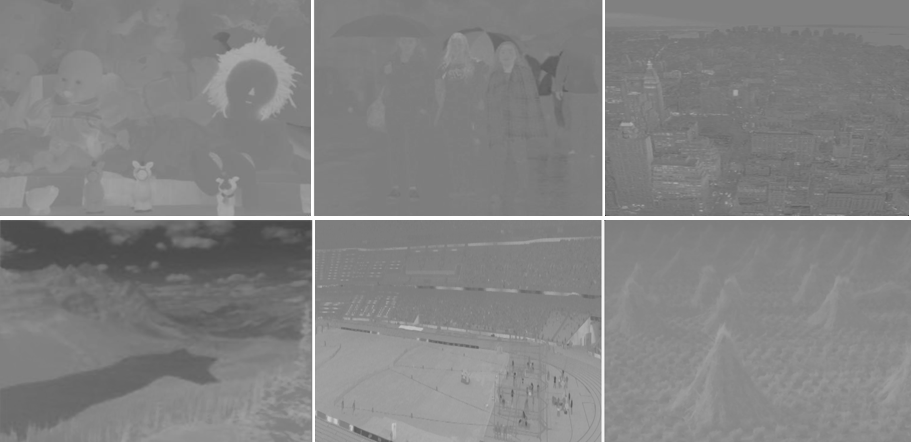
\includegraphics[width=1.0\linewidth]{30.png}
	\caption{Results of Color Channel a}
	\label{fig:15}
\end{figure*}
\subsection{Refinement of Luminance channel using median filter}
The channel $L$ indicates lightness on the Lab color channel. Median filtering is a nonlinear technique used to
expel noise from images. It is broadly utilized as it is extremely viable at expelling clamor while safeguarding
edges. The fundamental aim of the median filter is to go through the flag section by passage, supplanting every
section with the middle of neighboring passages.
\begin{figure*}
	\centering
	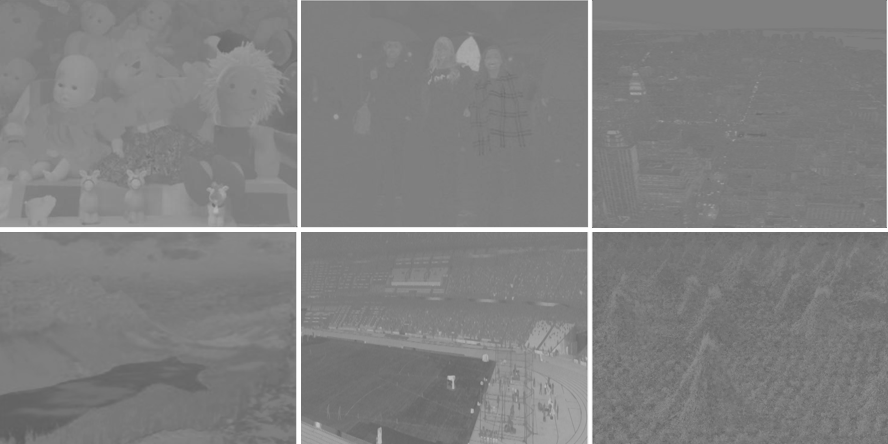
\includegraphics[width=1.0\linewidth]{31.png}
	\caption{Results of Color Channel b}
	\label{fig:16}
\end{figure*}

 The median filter considers every pixel in the image thus and takes a gander at its adjacent neighbors to choose whether or not it is illustrative of its environment. Rather than basically supplanting the pixel esteem with the mean of neighboring pixel values, it replaces it with the middle of those qualities. The middle is figured by first sorting all the pixel values from the encompassing neighborhood into numerical request and afterward supplanting the pixel being considered with the center pixel esteem. The median filtering output is given us\citing{a109}:
\begin{equation}
g(x,y)= med{f(x-i,y-j)i,j \varepsilon W}
\end{equation} 
where f(x,y), g(x,y) are the original image and the output image respectively, W is the two dimensional mask: the mask size is $nxn$ (where n is commonly odd) such as 3x3, 5x5, the mask shape may be linear, square, circular, cross. Figure~\ref{fig:17} shows the experimental results of the refined channel $L$

\begin{figure*}[!htb]
	\centering
	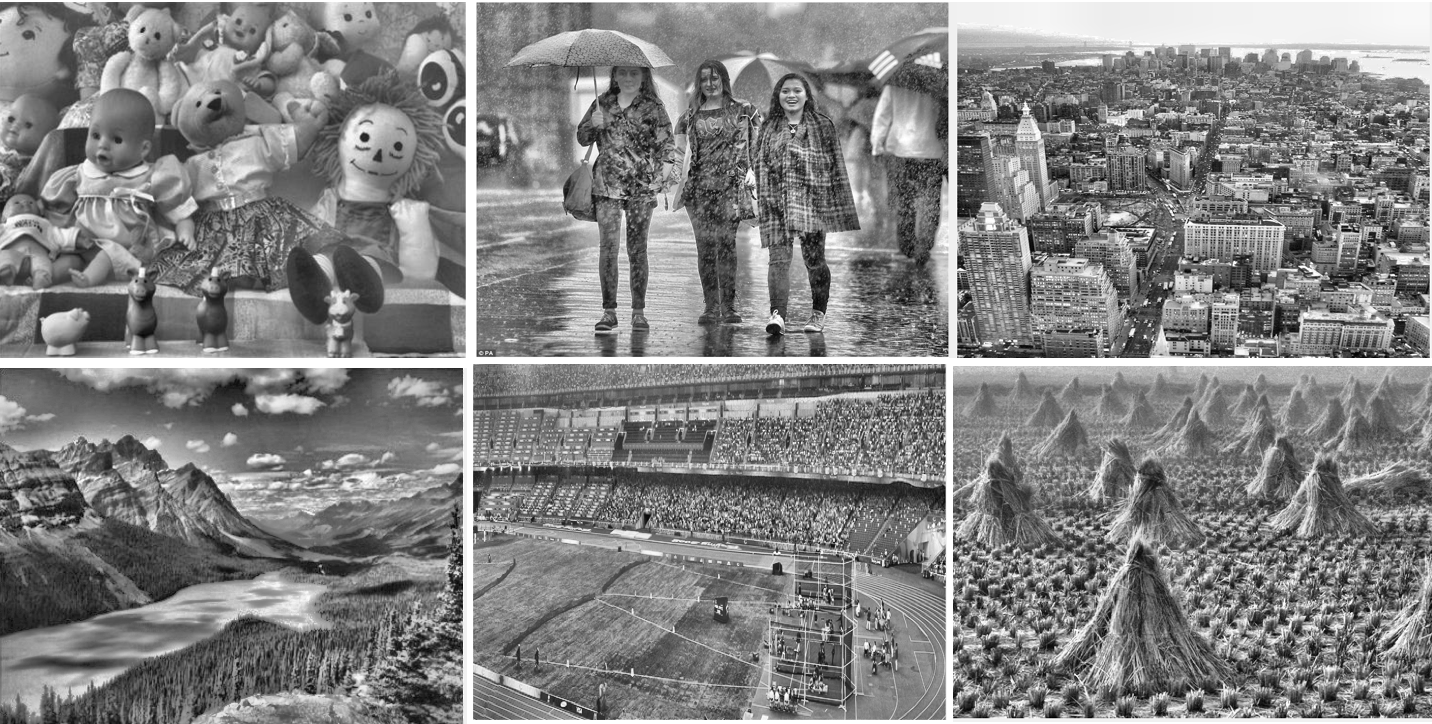
\includegraphics[width=1.0\linewidth]{32.png}
	\caption{Results of Luminance Channel L.}
	\label{fig:17}
\end{figure*}
\subsection{The Noise-Reducing Performance of the Median Filter:}
The removal of noise from an image is imperative in field image processing. Images are altered by an unforeseen shift in pixel intensity, brilliance, or low contrast, and as a result, they cannot be adopted immediately. Therefore, it is essential to discard the noise shown in an image. Since the median filter is a nonlinear channel, its scientific investigation is moderately complex for irregular clamor images. For an image with zero mean noise under normal distribution, the median filtering noise variance is approximately\citing{a110}. This thesis adopts a two phase technique to recognize the distorted pixel existing in the input image to generate a noise free image as an output image. The phases are the detection stage, which is reliable for identifying degraded pixels existing in the input image, and the Filtering stage, which is responsible for removing corrupted pixels. In this dissertation, we adopt a median-based technique using pixel correlation, i.e., the median value of neighboring pixels substitutes the damaged pixels. Before applying to filter, all pixels in the image have to be arranged in either ascending or descending order.  
\begin {equation} 
\sigma^2_m = \frac{1}{4_n f^2 \bar{(n)}} \approx \frac{\sigma^2_i}{n+ \frac{\pi}{2}-1}\cdot\frac{\pi}{2^.} \end{equation} 
where $\sigma^2_i$ is the input  noise  power (the variance), $n$ is  the  size  of  the  median  filtering  mask, $ f \bar{(n)} $   is  the function of the noise density. And the noise variance of the average filtering is defined as follows:
\begin{equation} \sigma^2_0 = \frac{1}{n} \sigma^2_i \end{equation}
Looking at  (7) and (8), the median filtering impacts rely on two things: (I) Extent of the veil (II) Dispersion of the noise. The median filtering execution of arbitrary noise decrease is superior to anything than the normal filtering execution, yet to the drive noise, particularly limited pules are more distantly separated and the  width is under $\frac{n}{2}$, the median filter is extremely effective.

\section{Experimental Results}
In this section, we evaluate our method against several state-of-the-art algorithms focusing on subjective analysis and computational run time. Our experiment implemented the proposed method on a Windows 7 64-bit operating system platform, Intel i5-4590 3.30GHz Core quad-core, 8 G of memory. We sample 50 hazy images from various datasets and perform experiments on them. Due to limited space, only some of the samples Figure~\ref{fig:13}. The proposed method's efficiency in this dissertation is compared to traditional dehazing algorithms such as  Fattal\citing{a31}, Kop\citing{a25} and Kratz\citing{a32} as shown in Figure~\ref{fig:19}  
\subsection{Qualitative Comparison}
In this section, we performed comparisons on the real-world hazy images obtained from the Internet.  Figure ~\ref{fig:19} illustrates samples of observations on real-world images in comparison with traditional  dehazing methods such as Fattal\citing{a31}, Kop\citing{a25} and Kratz\citing{a32}. At an initial glimpse, we recognize that most methods eliminated haze from images efficiently. However, under further examination, it is obvious that our method's subjective visual results are dim and there are many colour bands in the grey sky regions and halos on the edges of high buildings as shown in Figure~\ref{fig:19}(f1 -f3). Furthermore, the results are over-saturated because we do not employ the physical model to retrieve the haze free image. From Figure~\ref{fig:19}(d1-d3) Kratz\citing{a32} method still has some extra haze in distinctive regions (e.g., Forest images) and they appear darker. In Kop\citing{a25} results, images appear to contain halo artefacts caused by edge-deformation. Furthermore, the images appear over-saturated. In Fattal\citing{a31} due to colour variance and dense haze, the resultant image is not clear after dehazing and this method cannot dependable estimate transmission.


\begin{figure*}
	\centering
	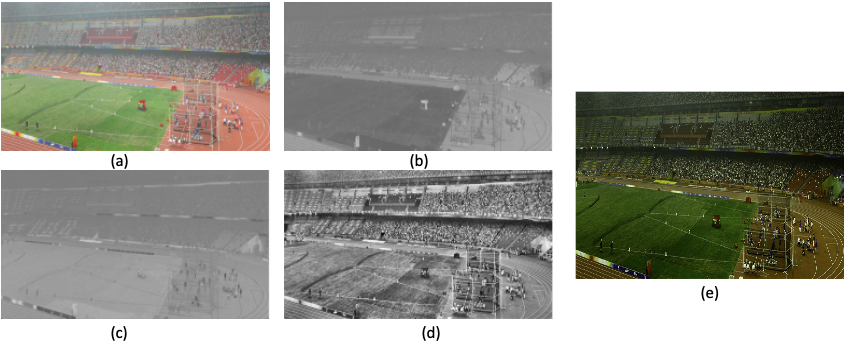
\includegraphics[width=1.0\linewidth]{33.png}
	\caption{Sample dehazing result using football park. (a) Input hazy image. (b) channel $b$. (c) Channel $a$. (d) Channel $L$. (e) Dehazed result}
	\label{fig:18}
\end{figure*}

\begin{table}
	\centering
	\caption{The objective image quality comparison of dehazing results - Figure~\ref{fig:19}. The value in the table are averages of all images}
    \begin{tabular}{|p{52pt}|p{58pt}|p{58pt}|p{58pt}|p{58pt}|p{52pt}|p{52pt}|p{52pt}|}
    
	\hline\textbf{Parameters}	& \textbf{Fattal's method[54]}& \textbf{Kop's method[43]} &  \textbf{Kratz's method[55]} &  \textbf{Proposed Method}\\
	\hline
	PSNR&  28.932 & \textbf{31.042} & 26.543 & 29.432\\
		\hline	
	SSIM&\textbf{0.491} & 0.535 & 0.678 & 0.5912\\
		\hline	
	$e$& 12.792 & \textbf{26.914}  & 15.583 & 15.672 \\
     	\hline	
	$\bar r$& \textbf{0.132} & 0.005 & 0.008 & 0.012\\
		\hline	
	$\sigma$& 0.132 & \textbf{0.005} & 0.008& 0.012\\
		\hline	
	contrast gain& 0.857 & 0.765 & 0.492 & \textbf{0.866}\\
	\hline	
\end{tabular}
	\label{Tab7}
\end{table}
\subsection{Quantitative Evaluation}
We evaluate our algorithm's dehazing performance on a synthetic dataset and compare the proposed method with state-of-the-art methods, including Fattal\citing{a31}, Kop\citing{a25} and Kratz\citing{a32}. This work adopts a blind evaluation approach to measure the contrast of an image before and post-processing. The method uses six parameters: (I) the new apparent edge ratio $e$, (II) normalize gradient of the visible edge $\bar r$, (III) proportion of saturated white or black pixels $\sigma$, (IV) Peak Signal-to-Noise Ratio (PSNR), (V) Structural Similarity (SSIM) and (VI) Contrast gain as shown in Table~\ref{Tab7}.

\begin{figure*}
	\centering
	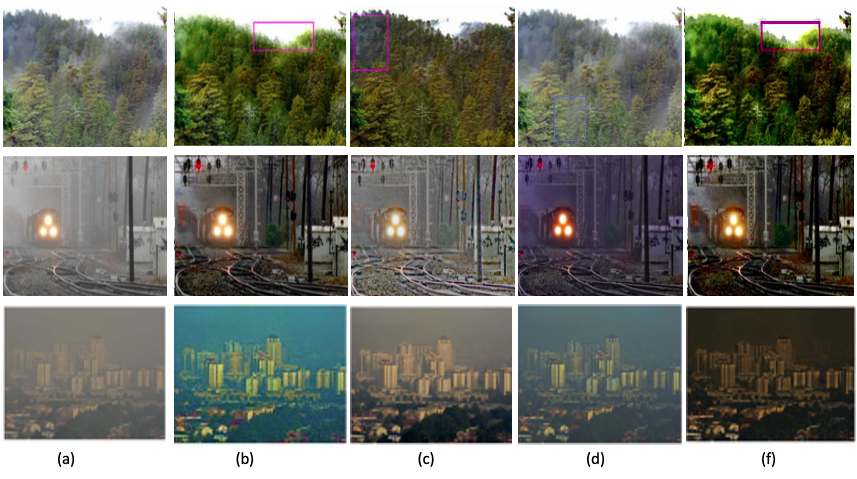
\includegraphics[width=1.0\linewidth]{34.png}
	\caption{Comparisons of traditional dehazing algorithms versus the proposed method. (a) Input hazy image. (b) Fattal [54] (c) Kop[43] (d) Kratz [55] (e) Our result}
	\label{fig:19}
\end{figure*}
The first two signs $(e, \bar r )$ of the blind assessment use the enhanced degree of image edges to describe the improved degree of the image clarity.  $e$ indicator is adopted to assess the colour restoration performance of defogging algorithms. 
\begin{equation}
e=\frac{n_r-n_o}{n_0}
\end{equation}
\begin{equation}
\bar r= exp\bigg(\frac{1}{n_r}\sum_{pi\epsilon\psi r} log r_i\bigg)
\end{equation}
\begin{equation}
\sigma=\frac{n_s}{dim_x +dim_y}
\end{equation} 
As shown in Table~\ref{Tab7}, a more extensive $e$ and $\bar r $ and a smaller $\epsilon$ denote  high quality dehazed image. PSNR is a full reference evaluation method, which uses three parameters:(I) the new apparent edge ratio (II) normalize gradient of the visible edge and the (III) proportion of saturated white or black pixels. This method demands clear images, and the photos to be evaluated. We define PSNR  as:
\begin{equation}
	PSNR = 10log_{10} \frac{ 255  }{\sqrt\big| X_{in}-X_{out}\big|^2}
\end{equation}

where $X(in)$ and $X(out)$ represent the hazy output and the hazy image model respectively. A dehazed image with a high contrast depict a unique algorithm. SSIM evaluation method, measures the similarities between the clean image and the image in three ways: (I) brightness, (II) contrast, and (III) structure. The definition of SSIM is as follows:

\begin{equation}
	SSIM= \frac{(2\mu_{ x_{in}}\mu _{x_{out}}+ \theta _2) (2 \sigma _{x_{in} x_{out}}+ \theta _2)}  { ( \mu ^2_{ x_{in}}+ \mu^2_{x_{out}}+ \theta_1)( \sigma^2_{x_{in}} +\sigma^2_{x_{out}} +\theta_1)      }
\end{equation}

where $\theta_1$ and $\theta_2$ are constant values utilized in the avoidance framework vulnerability created by a denominator of 0 with a  value range of [0,1]. A large value represents higher similarities between the ground truth and dehazed image. $\mu_{ x_{in}}$ and $ \mu_{ x_{out}}$ are the average of the hazy image output $ x_{in} $ and the hazy image model $x_{out}$ respectively. $\mu^2_{x_{in}}$ is the variance  of $ x_{in} $ . $ \mu^2_{x_{out}}$ is the variance of the hazy image model $x_{out}$.
Jobson et al.\citing{a111} introduced a visual contrast measure (VCM) to quantify the degree of the clarity of the image and is estimated as : 
\begin{equation}
VCM=100*R_v/R_t,
\end{equation}
where $R_v$ is the number of local areas, the standard deviation of which is larger than the given threshold, and Rt is the local regions' total number. The VCM uses the local standard deviation, which denotes the image's contrast, to measure the visibility. Overall, the higher the VCM, the clearer the improved image.
\begin{figure*}
	\centering
	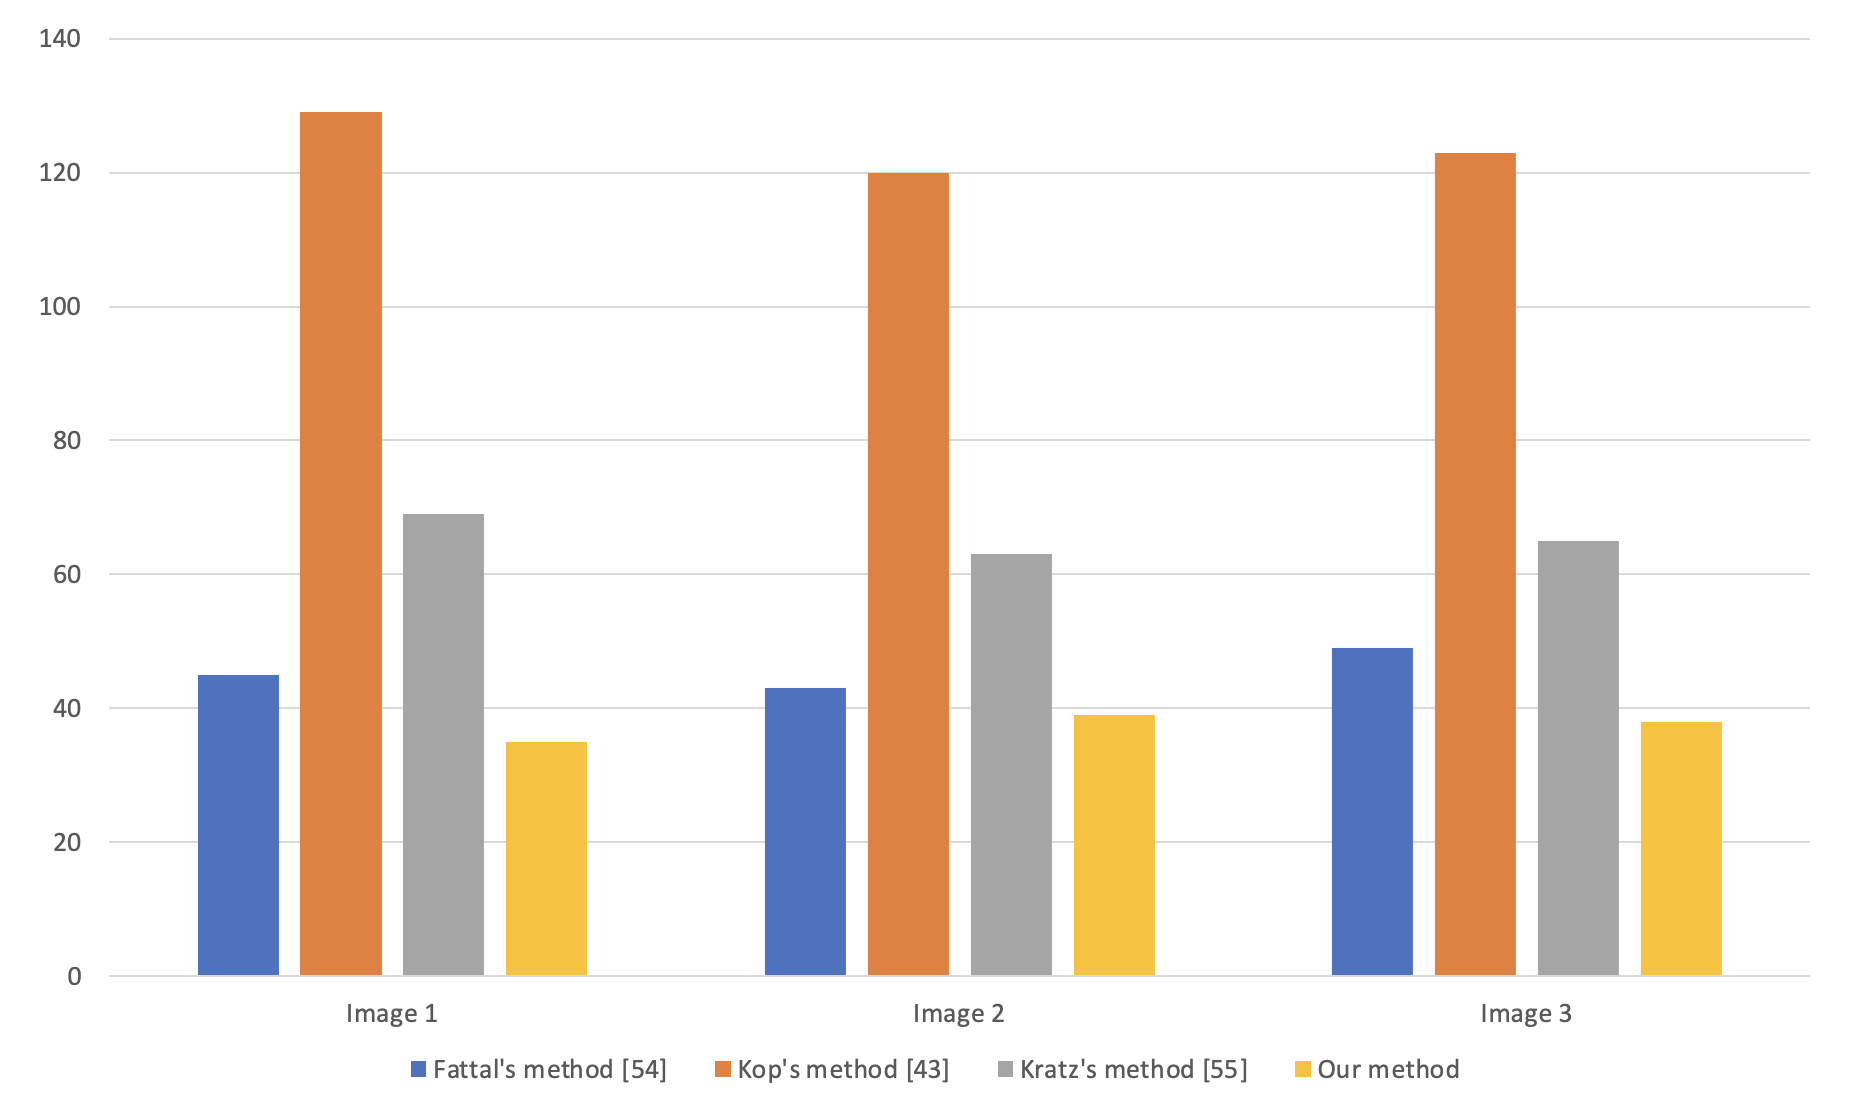
\includegraphics[width=1.0\linewidth]{36.png}
	\caption{Comparisons of traditional dehazing algorithms based on computational time complexity. Average time is measured in seconds}
	\label{fig:20}
\end{figure*}

From Table~\ref{Tab7}, we observe that the contrast of a clear image is usually much higher than that of a hazy image. Our method obtained the best result in contrast enhancement, followed by Fattal's method\citing{a31}.  However, the main focus of this work is on computational time complexity. Fattal's method\citing{a31} is a more simplistic and practical algorithm for magnifying dark and homogeneous hazy images. Kratz\citing{a32} algorithm achieved smaller values of all visibility assessment criteria than other dehazing algorithms. 

\subsection{Computational Run time}
To further show the effectiveness of the proposed method, we present a computational time comparison, as shown in Figure ~\ref{fig:20}
As compared to traditional methods Fattal\citing{a31}, Kop\citing{a25} and Kratz\citing{a32}, it is apparent that the subjective visual results of our approach are darker, notwithstanding that this work focuses on the computational time involved in single image dehazing. The findings prove that in producing a quality dehazed image, the proposed method consumes relatively low processing time compared with state-of-the-art methods. However, since other focuses on visual effects their computational time is very high. 

\section{Summary}
In this chapter, we propose a simple but effective novel
method for single image dehazing. The chapter focused on converting the hazy RGB image into Lab image. A manipulation analysis is applied on the various Lab color channels using CLAHE and median filter. Experimental results shows that this method functions admirably with bright dense hazy images. This approach functions admirably with very dense haze. However, results are often dim and lacks brightness because the method does not utilize a physical model to recover image. This method achieves a short computational time as compared to traditional method. \textbf{Published in the Proceedings of the 3rd International Conference on Multimedia and Image Processing }







\chapter {Conclusion and Future Works}
\label{Ch3}
Outdoor images are affected by natural and artificial adverse weather conditions such as mist, smoke, haze, fog, and smog due to the discernibility diminishing aerosols, which substantially cause a color change, image degradation, and scene darkening, among others. These aerosols are the arrangement of solid or fluid particles suspended by a blend of gases. Image dehazing has two main principal goals: (1) enhancing scene perceivability and amending the loss of light force caused by apparent aerosols. (2) Improving photography and computer vision application. However, dehazing is a challenging problem for image processing and the computer vision domain because of its dependence on the unknown scene depth. In this dissertation, we have studied the haze removal problems and related issues. This chapter presents the conclusion and summary of the contributions in this dissertation. Also, future research directions are discussed in this chapter.


\section{Concluding Remarks}
With digital imaging technology development, single image haze removal has become ubiquitous with the prior and neural network-based algorithms. It is urgent to improve and extend the current research in hazy digital images to achieve haze free images. This thesis has addressed removing haze from a single image with three novel contributions. The core contribution of this thesis is in three folds:
\begin{enumerate}
   \item Chapter one initially postulates the haze degradation model's research background and draws a comprehensive plan of this thesis. Subsequently, we register all the novel contributions of the present Ph.D. thesis that gave commencement to publication, demonstrating the essence and the authenticity of the work presented in this dissertation. 
   \item In Chapter two, we review the previous works on haze removal. We investigate multiple image, single image, and CNN based cases on their advantages and limitations. 
 
    \item  In Chapter Three, we proposed an algorithm based on strong prior using a solid mathematical foundation. The core contribution is twofold: (I) improve the estimation of transmission map and atmospheric light and (II) reduce computational complexity. The framework of the algorithm relies on DCP and Rayleigh scattering, which have solid mathematical foundations. The atmospheric light is estimated first by eliminating the block effect by selecting pixels with the highest intensity in the blue channel of the input image. To further eliminate unwanted texture information from the first step, the lowest pixel average in the Red and Green channel is computed. Finally, we obtain the atmospheric light by aggregating the first and second steps. The proposed method uses the Rayleigh scattering to calculate the scattering coefficient used in computing the transmission map.  Finally, a qualitative and visual effects comparison shows that the proposed method can effectively dehaze. The proposed method also has low computational consumption that shortens the processing time. Even though this approach is simple, the algorithm achieves excellent results. However, our approach still has some limitations: (I) a small percentage of artifacts exits in the dehazed image, and (II) extensive optimization of the transmission map is needed. Thus, there is the motivation for future research.
    
    \item In chapter four, we presented a residual based network for single image dehazing. Single image dehazing aiming to retrieve clear images from obscure images acquired under these conditions is an ill posed problem. Although many traditional methods have efficiently committed to annihilating haze, they pose some limitations due to their hand crafted features, e.g., dark channel, maximum contrast, and color disparity. The core contribution is to advance the transmission map estimation and atmospheric light using an end-to-end network. The overall architecture comprises four sequential modules: (I) feature extraction layer, which uses 2D convolution kernels to obtain information from the input image. (II) multi scale context aggregation, which adopts enlarged convolution to retrieve valuable highlights in various receptive fields without dissipating resolution, (III) residual network reduces the loss of extracted data while increasing the network vital level features. (IV) fully connected layers. Our algorithm’s framework does not depend on the physical model. However, it efficiently eliminates haze from an input image as opposed to traditional dehazing algorithms. The network learns by minimizing the mapping relationship between the RGB value and its respective transmission medium. Finally, to assess our method robustness, we generate outdoor and indoor synthetic hazy images using the NYU2 dataset. We generate datasets to train the proposed network from clear photos and their respective transmission map by simulating the physical model. Comparing experimental results with traditional dehazing algorithms reveals that the proposed method can effectively produce a significant enhancement in hazy regions.
    
    
    \item  In chapter five, we proposed a simple but effective novel method for single image dehazing.  Images acquired by the visual framework are genuinely corrupted under cloudy and foggy climate, affecting detection, tracking, and image recognition. Thus, restoring the actual scene from a hazy image is of great significance. The chapter presented a real time effective dehazing algorithm for hazy surveillance images to solve this problem. The chapter focused on converting the hazy RGB image into Lab image. A manipulation analysis is applied on the various Lab color channels using CLAHE and median filter. Experimental results show that this method functions admirably with bright, dense, hazy images. This approach functions admirably with a very dense haze. However, results are often dim and lack brightness because they do not utilize a physical model to recover the image. This method achieves a short computational time as compared to the traditional method. 


\end{enumerate}

\subsection{Limitation}
In chapter three, the proposed algorithm’s main limitation is categorized into two: (I) a small percentage of artefacts exits in the dehazed image, and (II) extensive optimization of the transmission map is needed. Thus, the motivation for future research. In chapter four, our proposed method trains on a set of the synthetic dataset generated using the haze physical model, which does not account for nighttime hazy images. Therefore, the proposed method is less effective in removing nighttime images with haze. Furthermore, due to the heterogeneous nature of extracting characteristics and estimating the transmission map using an end-to-end network, the computational time is high. Finally, in chapter five, the proposed algorithm's result is often dim and lacks brightness because it does not utilize a physical model to recover the image. This method achieves a short computational time as compared to the traditional method。 

\section{Suggestions for Future Works}
In the future, we intend to study the problem under more common hazy image conditions, e.g., spatially varying aerial light or channel conditional transmission. The dilemma becomes ill posed, and original priors are needed. In computer vision, we anticipate building a model to describe haze study quantitatively. Future research will also focus on how to reduce computational time and address nighttime hazy images using the CNN algorithm. This thesis refined the transmission map using the fast guided filter. This approach reduced the computational time associated with the traditional method. This strategy still needs additional research and improvement. Future research will develop a new filter to refine the transmission map in a more straightforward and time efficient way. Real­time computation is an essential thing in image dehazing.
\thesisacknowledgement
A doctoral thesis is often described as a solitary endeavour; however, this PhD thesis is the output of the effort and support of several people I am incredibly grateful for.
First and foremost, I would like to thank God, whose many blessings have brought me this far. I want to express my profound and earnest appreciation to my research Super­ visor, Professor ******. I appreciate all his contributions of time, ideas, and funding in making my PhD experience productive and stimulating. The joy and enthusiasm for research were contagious and motivational, even during challenging times in my PhD pursuit. I am also very grateful to my former Masters degree advisor, Professor ******. Professor ****** has been of great help by providing scientific advice and encourage­ment during my graduate school career. I want to thank the rest of my pre-thesis defence committee: Professor ****** and ******. Their insightful comments and the tricky questions incented me to widen my research from various perspectives.\par
I gratefully acknowledge the funding sources that made my PhD work possible. My publications were funded by THE SCIENCE AND TECHNOLOGY PROJECT OF SICHUAN 2020 under grant number 2020YFG0300 and Sichuan Province Science and Technology Support Program, under grant No. 2016GZ0073.\par
My experience at the University of Electronic Science and Technology China was made pleasant primarily due to friends and groups that became a component of my life. I am grateful for the time spent with ******************.\par
Lastly, my very profound gratitude goes to my parents, ************************, thank you for providing me unfailing backing and constant support throughout my years of study and through the process of researching and writing this thesis. I dedicate this thesis to my parents.

\nocite{*}
\thesisloadbibliography{emmathesis}

%
% Uncomment following codes to load bibliography database with native
% \bibliography command.
%
%\nocite{*}
%\bibliographystyle{thesis-uestc}
%\bibliography{reference}
%

\thesisappendix
\thesisloadaccomplish{publications}

\end{document}
